\documentclass[11pt]{article}

\usepackage[a4paper,margin=2.7cm]{geometry}
\usepackage[T1]{fontenc}
\usepackage[utf8]{inputenc}
\usepackage{lmodern}

\usepackage{amsmath,amssymb,amsthm}
\usepackage{booktabs}
\usepackage{graphicx}
\usepackage{float}
\usepackage[justification=raggedright,singlelinecheck=false]{caption}
\usepackage[numbers,sort&compress]{natbib}
\usepackage{placeins}
\usepackage{hyperref}
\usepackage[nameinlink]{cleveref}

\graphicspath{{figures/}}
\setcounter{topnumber}{5}
\setcounter{bottomnumber}{3}
\setcounter{totalnumber}{6}
\renewcommand{\topfraction}{0.95}
\renewcommand{\bottomfraction}{0.85}
\renewcommand{\textfraction}{0.05}
\renewcommand{\floatpagefraction}{0.75}
\setlength{\textfloatsep}{10pt plus 2pt minus 2pt}
\setlength{\floatsep}{8pt plus 2pt minus 2pt}
\setlength{\intextsep}{8pt plus 2pt minus 2pt}
\setlength{\abovecaptionskip}{4pt}
\setlength{\belowcaptionskip}{0pt}

\title{CARMA-Based Deseasonalization, Calibration and Pricing in Renewable Energy Markets}
\author{}
\date{\today}

\begin{document}

\maketitle

\begin{abstract}
\end{abstract}

\section{Introduction}\label{sec:introduction}

This paper builds a compact empirical framework for pricing renewable-energy
contracts whose payoffs depend jointly on German day-ahead electricity prices
and weather-driven production factors. The workflow first removes deterministic
seasonality from prices, temperature, solar capacity factors, and wind capacity
factors. It then fits marginal CARMA models to the resulting stochastic factors,
recovers their driving noises, and estimates one-way shock couplings from
temperature, solar, and wind into the price driver. The calibrated system is
then ready for joint simulation and pricing.

\section{Data and Deseasonalization}\label{sec:deseasonalization}

\subsection{Common Setup}\label{ssec:deseasonalization-common}

Each raw series is first mapped to a coordinate in which an additive model is
appropriate. Denote this transformed observable by \(Y^F_t\), where
\(F\in\{P,T,Q,W\}\) refers to price, temperature, solar, and wind. We write
\begin{equation}
  Y^F_t=\Lambda^F_t+X^F_t .
  \label{eq:deseasonalization-common-decomposition}
\end{equation}
Here \(\Lambda^F_t\) is a deterministic seasonal component and \(X^F_t\) is the
stochastic residual used in the CARMA calibration. This section specifies the
coordinate \(Y^F_t\), the seasonal structure used for \(\Lambda^F_t\), and the
diagnostic evidence left after deseasonalization. The remaining serial
dependence is then modeled stochastically.

For the physical factors \(T\), \(Q\), and \(W\), the seasonal component is a
linear regression on calendar and Fourier covariates after the relevant
transformation has been applied, with coefficients estimated by OLS. Prices use
a separate normalized seasonal construction, described below, because the
intraday price profile is more irregular.

\subsection{Electricity Prices}\label{ssec:price-deseasonalization}

We use hourly German day-ahead prices for the DE--LU bidding zone. The CARMA
calibration sample is 2023--2025 in UTC, while
\cref{fig:price-window-2021-2025} also shows 2021--2022. As seen in the figure,
the 2023--2025 window is used to exclude the exceptional price spikes associated
with the energy crisis and the war in Ukraine.

Since the spot price \(S_t\) can be negative, the stochastic price factor is
defined in shifted log coordinates,
\begin{equation}
  \widetilde S_t=\log(S_t+\delta),
  \qquad
  \delta=1000\ \text{EUR/MWh},
  \qquad
  S_t=\exp(\widetilde S_t)-\delta .
  \label{eq:price-log-shift}
\end{equation}
Thus \(Y^P_t=\widetilde S_t\). The price seasonality follows the
electricity-price deseasonalization approach discussed in \citep{Paraschiv2013}.
We estimate \(\Lambda^P_t\) with a multiplicative seasonal weight in log-price
coordinates,
\begin{equation}
  \widehat\Lambda^P_t=\bar p\,\widehat F^Y_{d(t)}\,\widehat F^D_t .
  \label{eq:price-seasonality}
\end{equation}
The daily factor \(\widehat F^Y\) is fitted from normalized daily mean
log-prices using weekday and month effects, with August split into early and
late subperiods. The intraday factor \(\widehat F^D\) is fitted from hour-of-day
profiles within 20 calendar classes, then normalized so that it only captures
shape. The estimated residual is the price factor used in the CARMA
calibration.

\begin{figure}[!htbp]
  \centering
  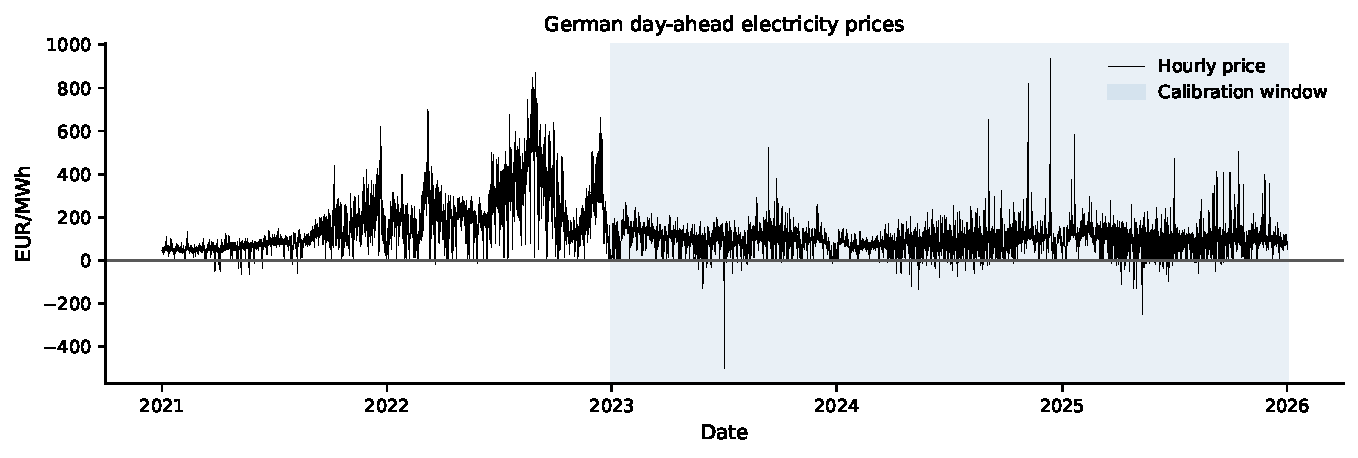
\includegraphics[width=0.97\textwidth]{deseasonalization/price_window_2021_2025.pdf}
  \caption{Hourly German day-ahead electricity prices from 2021 to 2025.
  The shaded region is the 2023--2025 calibration window.}
  \label{fig:price-window-2021-2025}
\end{figure}

\begin{figure}[!htbp]
  \centering
  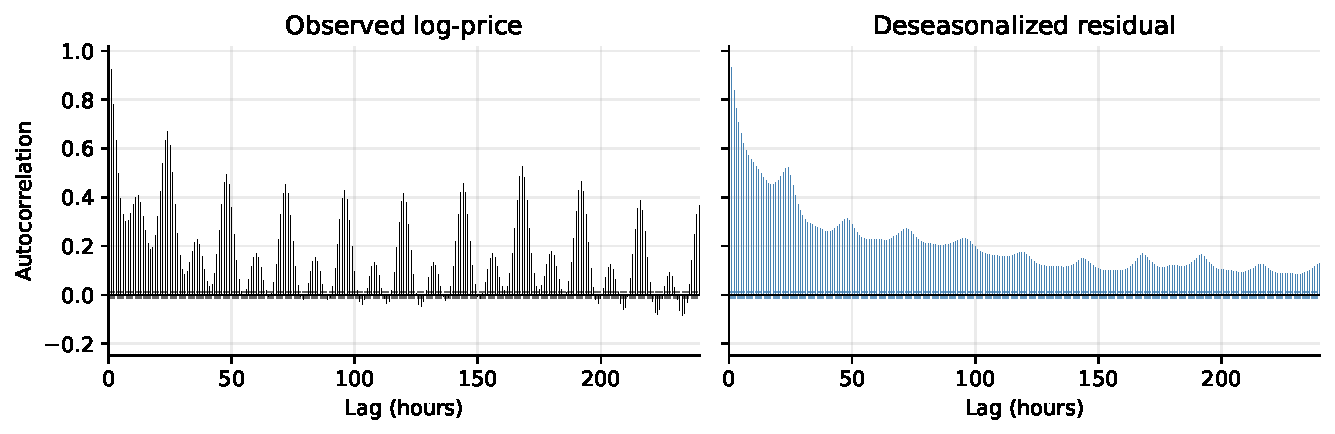
\includegraphics[width=0.97\textwidth]{deseasonalization/price_acf_before_after_240.pdf}
  \caption{Empirical autocorrelation of the shifted log-price and of the
  deseasonalized price residual over 240 hourly lags.}
  \label{fig:price-acf-before-after}
\end{figure}

\FloatBarrier

\subsection{Temperature}\label{ssec:temperature-deseasonalization}

We use hourly 2-meter Berlin temperature over the same 2023--2025 UTC sample.
No transform is needed, so \(Y^T_t=T_t\). The seasonal regression uses a compact
Fourier basis, where \(\tau_t\) denotes the elapsed number of hours and
\(P_y=365.25\times24\).
\begin{equation}
  \Lambda^T_t
  =
  \beta_0+\beta_1\tau_t
  +\sum_{k=1}^{3}\left[
    a_k(t)\cos\left(\frac{2\pi k\tau_t}{24}\right)
    +b_k(t)\sin\left(\frac{2\pi k\tau_t}{24}\right)
  \right]
  +a_y\cos\left(\frac{2\pi\tau_t}{P_y}\right)
  +b_y\sin\left(\frac{2\pi\tau_t}{P_y}\right).
  \label{eq:temperature-seasonality}
\end{equation}
The daily-cycle coefficients \(a_k(t)\) and \(b_k(t)\) are annual Fourier
functions, so the intraday temperature profile can vary smoothly over the year.
\Cref{fig:temperature-acf-before-after} shows the residual dependence left for
the CARMA model.

\begin{figure}[!htbp]
  \centering
  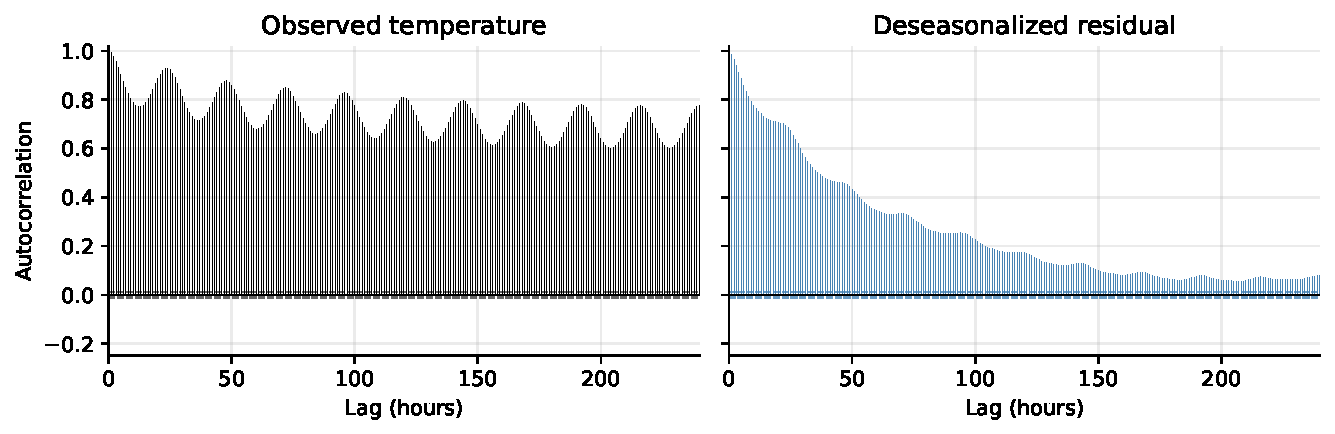
\includegraphics[width=0.97\textwidth]{deseasonalization/temperature_acf_before_after_240.pdf}
  \caption{Empirical autocorrelation of observed temperature and of the
  deseasonalized temperature residual over 240 hourly lags.}
  \label{fig:temperature-acf-before-after}
\end{figure}

\FloatBarrier

\subsection{Solar Capacity Factors}\label{ssec:solar-deseasonalization}

Let \(Q_t\in[0,1]\) be the German solar capacity factor. Solar cannot be treated
as a simple additive bounded process because production is structurally zero at
night and the daylight support changes over the year. We first estimate an
empirical clear-sky envelope \(\widehat C_t=\widehat C_{d(t),h(t)}\) from the
98\% quantile of \(Q_t\) by day-of-year and hour-of-day cells, with missing-cell
completion and circular 21-day smoothing.

The stochastic solar variable is defined as a clear-sky shortfall,
\begin{equation}
\begin{aligned}
  R_t
  =
  \operatorname{clip}_{[0,1]}
  \left(1-\frac{Q_t}{\max(\widehat C_t,10^{-4})}\right),
  \qquad
  Z_t
  &=
  \operatorname{clip}_{[10^{-4},1-10^{-4}]}
  \left(\frac{R_t-10^{-4}}{0.9998}\right),
  \\
  Y^Q_t
  &=
  \log\left(\frac{Z_t}{1-Z_t}\right).
\end{aligned}
\label{eq:solar-logit-transform}
\end{equation}
A positive solar latent shock therefore means larger cloudiness or solar
shortfall, not larger physical production. Deseasonalization is performed with
\(Y^Q_t\) as the transformed coordinate. The seasonal regression combines hour
and month effects, annual Fourier terms, and hour-by-annual interactions. We
write \(H_h(t)=\mathbf 1_{\{h(t)=h\}}\), \(M_m(t)=\mathbf
1_{\{\operatorname{month}(t)=m\}}\), and \(\phi_t=2\pi d(t)/365.25\). The
regression is
\begin{equation}
  \begin{aligned}
  \Lambda^Q_t
  =
  \gamma_0
  &+
  \sum_{h=1}^{23}\gamma_h H_h(t)
  +
  \sum_{m=2}^{12}\eta_m M_m(t)
  +
  \sum_{k=1}^{3}
  \left[
    a_k\cos(k\phi_t)+b_k\sin(k\phi_t)
  \right] \\
  &+
  \sum_{h=1}^{23}H_h(t)
  \sum_{k=1}^{2}
  \left[
    u_{h,k}\cos(k\phi_t)+v_{h,k}\sin(k\phi_t)
  \right].
  \end{aligned}
  \label{eq:solar-seasonality}
\end{equation}
For physical diagnostics, the fitted latent seasonality is mapped back through
the inverse clear-sky transform.

\begin{figure}[!htbp]
  \centering
  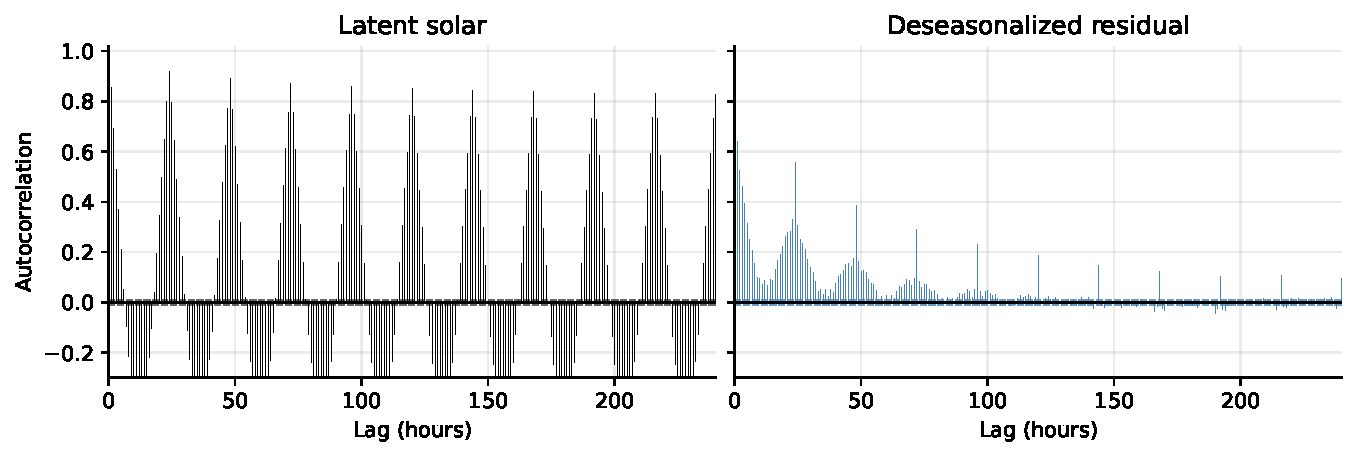
\includegraphics[width=0.97\textwidth]{deseasonalization/solar_acf_before_after_240.pdf}
  \caption{Empirical autocorrelation of the latent solar coordinate and of the
  deseasonalized solar residual over 240 hourly lags.}
  \label{fig:solar-acf-before-after}
\end{figure}

\FloatBarrier

\subsection{Wind Capacity Factors}\label{ssec:wind-deseasonalization}

Let \(W_t\in[0,1]\) be the German wind capacity factor, aligned with the price
calendar in UTC. Wind has no structural day-night support, but it is bounded and
persistent. We therefore work in logit coordinates,
\begin{equation}
  W^\varepsilon_t=\operatorname{clip}_{[10^{-4},1-10^{-4}]}(W_t),
  \qquad
  Y^W_t=\log\left(\frac{W^\varepsilon_t}{1-W^\varepsilon_t}\right),
  \qquad
  W_t=\sigma(Y^W_t).
  \label{eq:wind-logit-transform}
\end{equation}
The transform is monotone, so a positive wind latent shock corresponds to
higher-than-seasonal physical wind production. The seasonal regression includes
hour, weekday, month, and annual Fourier effects. Physical-scale diagnostics are
obtained by mapping \(\widehat\Lambda^W_t\) back through the logistic function.

\begin{figure}[!htbp]
  \centering
  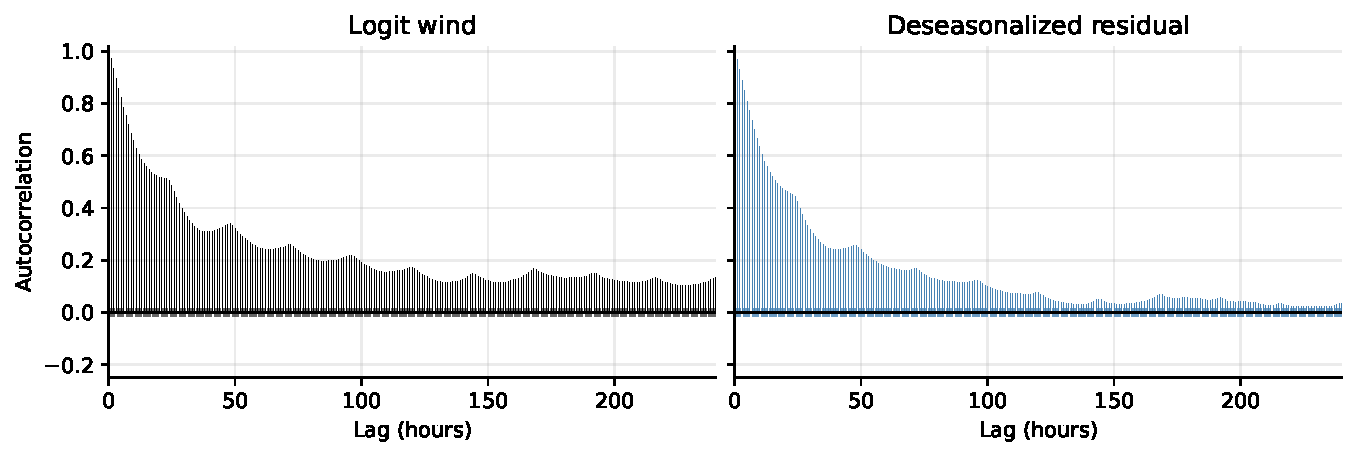
\includegraphics[width=0.97\textwidth]{deseasonalization/wind_acf_before_after_240.pdf}
  \caption{Empirical autocorrelation of the logit wind capacity factor and of
  the deseasonalized wind residual over 240 hourly lags.}
  \label{fig:wind-acf-before-after}
\end{figure}

\FloatBarrier

\section{Marginal CARMA Calibration}\label{sec:marginal-carma-calibration}

\subsection{Calibration Framework}\label{ssec:carma-calibration-framework}

Each deseasonalized marginal factor is modeled as a stationary Levy-driven
CARMA process in state-space form \citep{BrockwellLindner2024Ch18}. For a
CARMA\((p,q)\),
\begin{equation}
  dG_t=A G_t\,dt+e_p\,dL_t,
  \qquad
  X_t=b^\top G_t ,
  \label{eq:carma-state-space}
\end{equation}
where \(L\) is a one-dimensional Levy driver and \(A\) is the companion matrix
of
\begin{equation}
  a(z)=z^p+a_1z^{p-1}+\cdots+a_p .
  \label{eq:carma-ar-polynomial}
\end{equation}
The roots of \(a\) are required to have negative real parts. The moving-average
vector is written as \(b=(b_0,\ldots,b_q,0,\ldots,0)^\top\), with the last
non-zero coefficient normalized to one. Throughout the paper we use the full
moving-average convention \(q=p-1\), unless stated otherwise.

The order is initialized from the empirical autocorrelation function. A real
root contributes a monotone exponential decay, while a complex conjugate pair
contributes a damped oscillation. We therefore fit
\begin{equation}
  \rho_{\mathrm{ms}}(h)
  =
  \sum_{r=1}^{R} w_r e^{-\kappa_r h}
  +
  \sum_{\ell=1}^{C} w_{o,\ell} e^{-\kappa_{o,\ell}h}
  \cos(\omega_\ell h),
  \qquad
  \sum_r w_r+\sum_\ell w_{o,\ell}=1 ,
  \label{eq:carma-multiscale-acf}
\end{equation}
with non-negative weights. In the applications below there is one daily
oscillatory pair, with \(\omega=2\pi/24\), and the fitted ACF is spectrally
factorized to obtain a stable initial CARMA model.

Starting from this initialization, the final marginal parameters are estimated
by exact Gaussian prediction-error QMLE, following the Kalman likelihood
construction for sampled CARMA processes \citep{BrockwellLindner2024Ch19}. For
given CARMA coefficients, the Kalman recursion gives one-step prediction errors
\(e_i\) and innovation variances \(r_i\) under unit Levy variance. Since the
Levy drift enters as a constant mean shift, the adjusted innovation is
\[
  \varepsilon_i(m)=e_i-mc_i .
\]
The drift rate and variance rate are profiled as
\begin{equation}
  \widehat m
  =
  \frac{\sum_i e_i c_i/r_i}{\sum_i c_i^2/r_i},
  \qquad
  \widehat \nu^2
  =
  \frac{1}{n}\sum_i
  \frac{\varepsilon_i(\widehat m)^2}{r_i}.
  \label{eq:carma-qmle-profile}
\end{equation}
The optimized criterion is the reduced Gaussian prediction-error likelihood,
augmented when needed by a soft ACF penalty,
\begin{equation}
  \mathcal J(\theta)
  =
  \log(\widehat\nu^2)
  +
  \frac{1}{n}\sum_i \log r_i
  +
  \lambda_{\mathrm{acf}}
  \frac{1}{|H|}
  \sum_{h\in H}
  \omega_h
  \left(\rho_\theta(h)-\widehat\rho(h)\right)^2 .
  \label{eq:carma-qmle-objective}
\end{equation}
The penalty stabilizes long-lag dependence without replacing the likelihood
criterion. Its value is reported separately for each marginal.

Once the CARMA parameters are fixed, the hourly Levy increments are recovered
from the smoothed state path, as in the QMLE framework of
\citet{BrockwellLindner2024Ch19}. Let \(\widehat G_t\) denote the RTS-smoothed
state, including the profiled drift correction \(\widehat m(-A)^{-1}e_p\).
Choose a real root \(\lambda_r\) of \(a\), taken in practice as the slowest real
root, and let \(E\) be the matrix of companion eigenvectors. The corresponding
modal coordinate satisfies a scalar driven equation, giving
\begin{equation}
  \widehat Z_r(t)=b(\lambda_r)e_r^\top E^{-1}\widehat G_t,\qquad
  d\widehat Z_r(t)=\lambda_r\widehat Z_r(t)\,dt+\alpha_r\,dL_t,
  \qquad
  \alpha_r=\frac{b(\lambda_r)}{a'(\lambda_r)},
  \label{eq:levy-modal-recovery}
\end{equation}
and therefore
\begin{equation}
  \widehat L_t-\widehat L_0
  =
  \frac{\widehat Z_r(t)-\widehat Z_r(0)
  -\lambda_r\int_0^t \widehat Z_r(s)\,ds}{\alpha_r}.
  \label{eq:levy-driver-recovery}
\end{equation}
On the hourly grid the integral is evaluated numerically, and the empirical
driver sample used below is
\(\Delta\widehat L_i=\widehat L_{t_i}-\widehat L_{t_{i-1}}\).

\subsection{German Spot Prices}\label{ssec:german-price-carma-calibration}

The deseasonalized German log-price factor \(\widehat X^P\) is calibrated with
the procedure of \cref{ssec:carma-calibration-framework}. To represent a
decaying ACF with damped 24-hour oscillations, the initialization combines one
daily oscillatory pair with three real half-lives. The first real scale is
expected to be hourly, the second daily, and the third is fixed at 120 d during
initialization to impose a slow component for option-pricing horizons.
\begin{equation}
  \rho_{\mathrm{ms}}(h)
  =
  \sum_{i=1}^{3} w_i \exp(-\kappa_i h)
  +
  w_4 \exp(-\kappa_4 h)
  \cos\left(\frac{2\pi h}{24}\right),
  \qquad
  \sum_{i=1}^{4}w_i=1,\quad w_i\ge 0,
  \label{eq:price-multiscale-acf}
\end{equation}
Here \(h\) is measured in hours, and the oscillatory frequency is fixed at
\(2\pi/24\). The additional long real half-life is specific to the price
model. It is introduced only at initialization to keep slow price persistence
available for pricing, while the temperature, solar, and wind marginals below
do not require such an imposed long mode. The fitted decomposition has three
real roots and one complex conjugate pair, which gives the autoregressive order
\[
  p = 3 + 2 = 5 .
\]
We use the full moving-average order \(q=p-1=4\). Spectral factorization of the
fitted ACF then gives the initial CARMA(5,4) model.

\FloatBarrier

\begin{table}[!htbp]
  \centering
  \caption{German price CARMA(5,4) half-lives before and after penalized QMLE.}
  \label{tab:price-carma-half-lives}
  \begin{tabular}{@{}lll@{}}
    \toprule
    Root & Half-life after initialization & Half-life after QMLE \\
    \midrule
    \(\lambda_1\) & \(2.63\) h & \(4.52\) h \\
    \(\lambda_2\) & \(1.20\) d & \(1.50\) d \\
    \(\lambda_o\) & \(7.21\) d & \(7.21\) d \\
    \(\lambda_3\) & \(120\) d & \(82.4\) d \\
    \bottomrule
  \end{tabular}
\end{table}

\FloatBarrier

The QMLE step uses \(\lambda_{\mathrm{acf}}=10\). The daily pair remains fixed,
whereas the three real half-lives, including the slow one, and the
moving-average coefficients are re-estimated. The final log-likelihood is
\(77709\). As shown in
\cref{fig:price-spot-acf-calibration}, the ACF penalty keeps the final CARMA
autocorrelation close to the multiscale initialization while allowing the
likelihood to improve.

\begin{figure}[!htbp]
  \centering
  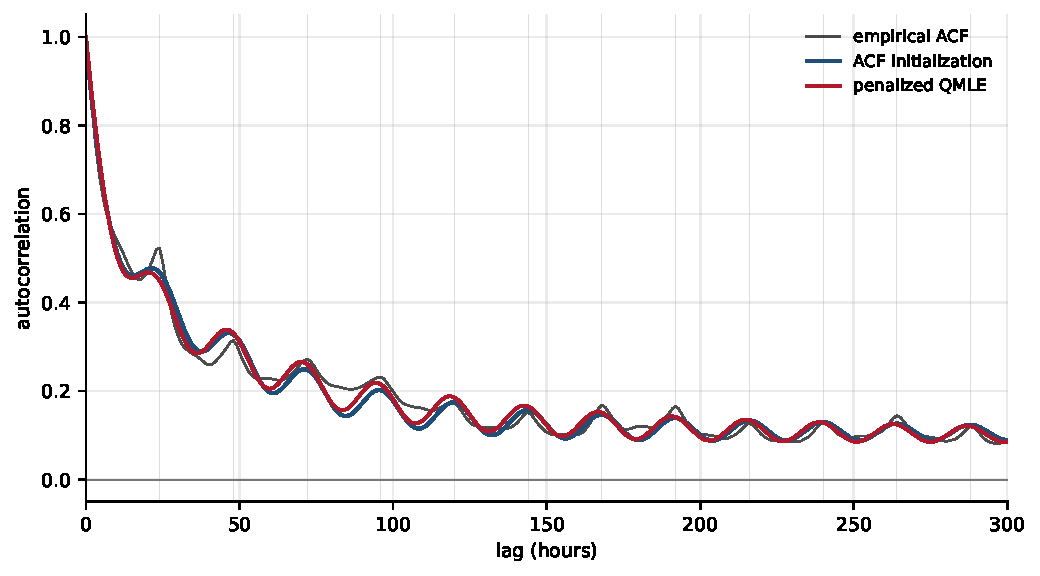
\includegraphics[width=0.78\textwidth]{calibration/price_spot_acf_calibration_300.pdf}
  \caption{German price ACF calibration over 300 hourly lags, comparing the
  empirical autocorrelation, the multiscale initialization, and the final
  CARMA(5,4) autocorrelation after QMLE.}
  \label{fig:price-spot-acf-calibration}
\end{figure}

\begin{table}[!htbp]
  \centering
  \caption{Gaussian log-likelihood comparison on the same deseasonalized German
  log-price residuals.}
  \label{tab:price-loglik-comparison}
  \begin{tabular}{@{}lr@{}}
    \toprule
    Model & Log-likelihood \\
    \midrule
    CARMA(5,4), ACF initialization & \(77562\) \\
    CARMA(5,4), QMLE & \(77709\) \\
    ARMA(1,0) & \(77454\) \\
    ARMA(5,4) & \(78661\) \\
    \bottomrule
  \end{tabular}
\end{table}

\Cref{tab:price-loglik-comparison} shows that the penalized QMLE improves the
Gaussian log-likelihood relative to the ACF initialization, although it remains
below the unconstrained ARMA(5,4) benchmark. Pure QMLE can increase this
likelihood further, as discussed below, but only by shortening the slow price
component too much.

\begin{figure}[!htbp]
  \centering
  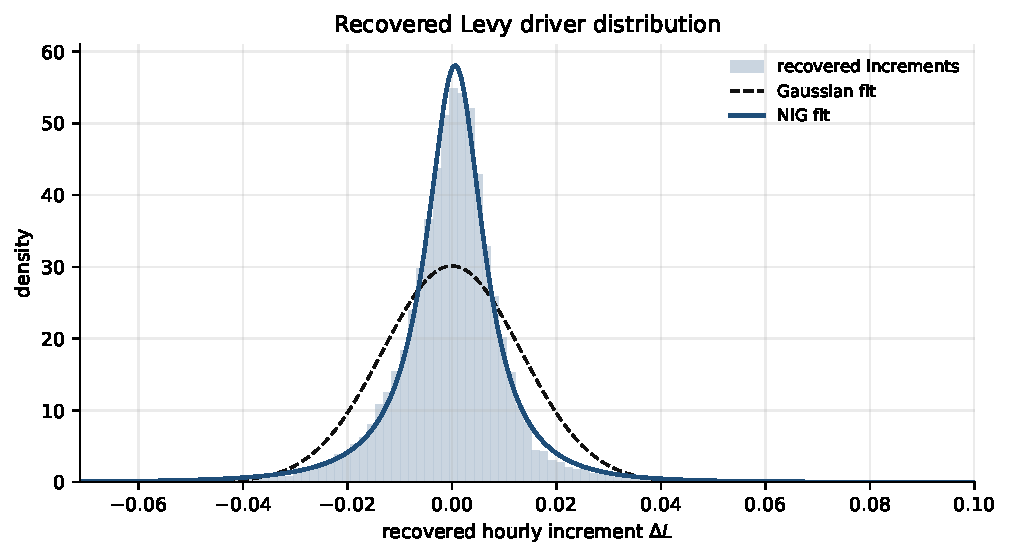
\includegraphics[width=0.70\textwidth]{calibration/price_spot_driver_distribution_fit.pdf}
  \caption{Recovered hourly Levy driver increments for the German price CARMA
  model, with Gaussian and NIG distribution fits.}
  \label{fig:price-spot-driver-distribution}
\end{figure}

After calibration, the driver increments recovered by
\cref{eq:levy-driver-recovery} are fitted with a Gaussian law and with a normal
inverse Gaussian law. The NIG specification is preferred according to the AIC
criterion, consistently with \cref{fig:price-spot-driver-distribution}. The NIG
density better matches the asymmetry and tail thickness of the recovered
increments than the Gaussian benchmark.

\begin{figure}[!htbp]
  \centering
  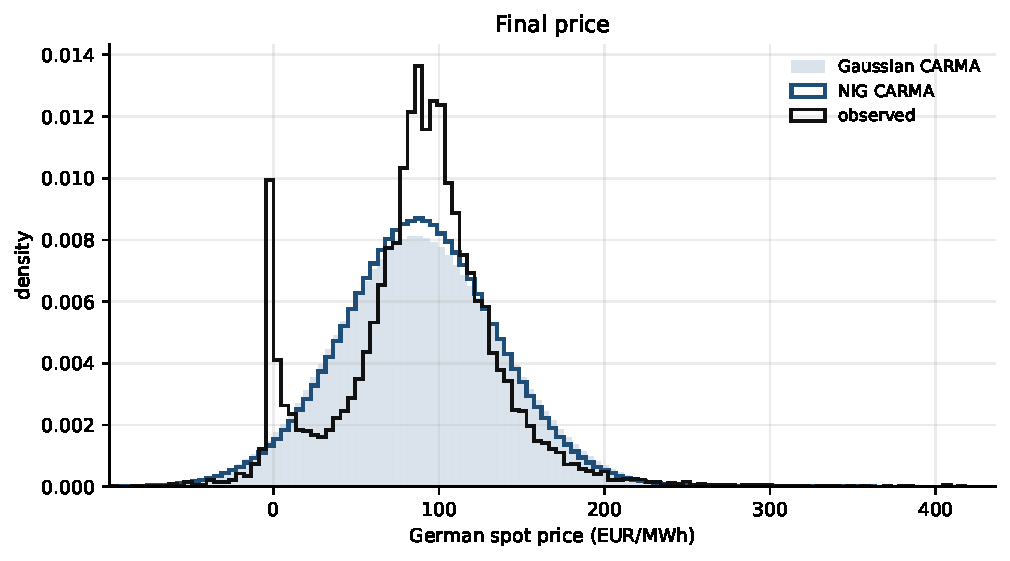
\includegraphics[width=0.74\textwidth]{calibration/price_spot_final_price_distribution.pdf}
  \caption{Distribution check for the final German spot price in EUR/MWh,
  comparing the observed data with prices simulated from the Gaussian and NIG
  CARMA marginals.}
  \label{fig:price-spot-final-price-distribution}
\end{figure}

\Cref{fig:price-spot-final-price-distribution} maps the simulated CARMA
residuals back to EUR/MWh using the same seasonal component. The NIG-driven
model improves the distribution relative to the Gaussian-driven model, but
neither specification reproduces the bimodality of the empirical price
distribution, in particular the concentration around zero EUR/MWh. In the
European day-ahead market, hourly prices are obtained by uniform-price auctions
from the intersection of aggregated supply and demand curves. During hours with
low residual demand, renewable production and other low marginal-cost or
must-run units frequently set, or strongly constrain, the clearing price near
zero. During tighter hours, the marginal unit is usually thermal or flexible
generation with a strictly positive bid. This market-clearing mechanism creates
regime-like mass in the final price distribution and cannot be reproduced by a
smooth continuous-time CARMA marginal factor alone.

We also ran a pure exact QMLE without the ACF penalty
\((\lambda_{\mathrm{acf}}=0)\), using semi-global restarts from the same
CARMA(5,4) structure. The best run over 20 restarts increases the Gaussian
log-likelihood because the objective only rewards one-step prediction fit. It
does not penalize the loss of long-lag ACF structure.

\begin{table}[H]
  \centering
  \caption{Penalized versus pure QMLE for the German price CARMA(5,4).}
  \label{tab:price-pure-qmle-comparison}
  \begin{tabular}{@{}lcc@{}}
    \toprule
    Quantity & Retained QMLE & Pure QMLE \\
    \midrule
    ACF penalty \(\lambda_{\mathrm{acf}}\) & \(10\) & \(0\) \\
    Log-likelihood & \(77709\) & \(78808\) \\
    \(\lambda_1\) half-life & \(4.52\) h & \(0.510\) h \\
    \(\lambda_2\) half-life & \(1.50\) d & \(1.20\) h \\
    \(\lambda_o\) half-life & \(7.21\) d & \(5.20\) d \\
    \(\lambda_3\) half-life & \(82.4\) d & \(1.40\) d \\
    \bottomrule
  \end{tabular}
\end{table}

The pure QMLE is therefore better as a one-step Gaussian likelihood fit, but it
collapses the slow price factor from several months to about one day. This
choice is not appropriate for the pricing step, because the model would lose the
long-horizon persistence imposed by the ACF initialization and retained by the
penalized QMLE.

\FloatBarrier

\subsection{German Temperature}\label{ssec:german-temperature-carma-calibration}

The stochastic temperature factor \(\widehat X^T\) is the hourly Berlin
temperature residual after deterministic Fourier deseasonalization. It is
modeled with the stationary CARMA structure of \cref{eq:carma-state-space}. Its
empirical ACF is smoother than the electricity price ACF, but it still contains
a daily oscillatory component. The initialization therefore uses two real modes
and one daily pair.
\begin{equation}
  \rho_{\mathrm{ms}}^T(h)
  =
  w_f e^{-\kappa_f h}
  +
  w_s e^{-\kappa_s h}
  +
  w_d e^{-\kappa_d h}
  \cos\left(\frac{2\pi h}{24}\right),
  \qquad
  w_f+w_s+w_d=1,\quad w_f,w_s,w_d\ge 0 .
  \label{eq:temperature-multiscale-acf}
\end{equation}
The two real components represent a relatively fast decay and a slower
persistent component, while the complex conjugate pair enforces the 24-hour
oscillation. The resulting order is
\[
  p = 2 + 2 = 4,
  \qquad q=p-1=3 .
\]
The daily frequency is fixed in the ACF step and the daily AR pair is kept fixed
in QMLE. The two real AR roots and the moving-average polynomial are
re-estimated.

\FloatBarrier

\begin{table}[!htbp]
  \centering
  \caption{German temperature CARMA(4,3) half-lives before and after penalized
  QMLE.}
  \label{tab:temperature-carma-half-lives}
  \begin{tabular}{@{}lll@{}}
    \toprule
    Root & Half-life after initialization & Half-life after QMLE \\
    \midrule
    \(\lambda_1\) & \(1.06\) d & \(0.530\) h \\
    \(\lambda_2\) & \(2.42\) d & \(1.59\) d \\
    \(\lambda_o\) & \(3.03\) d & \(3.03\) d \\
    \bottomrule
  \end{tabular}
\end{table}

\FloatBarrier

\begin{figure}[!htbp]
  \centering
  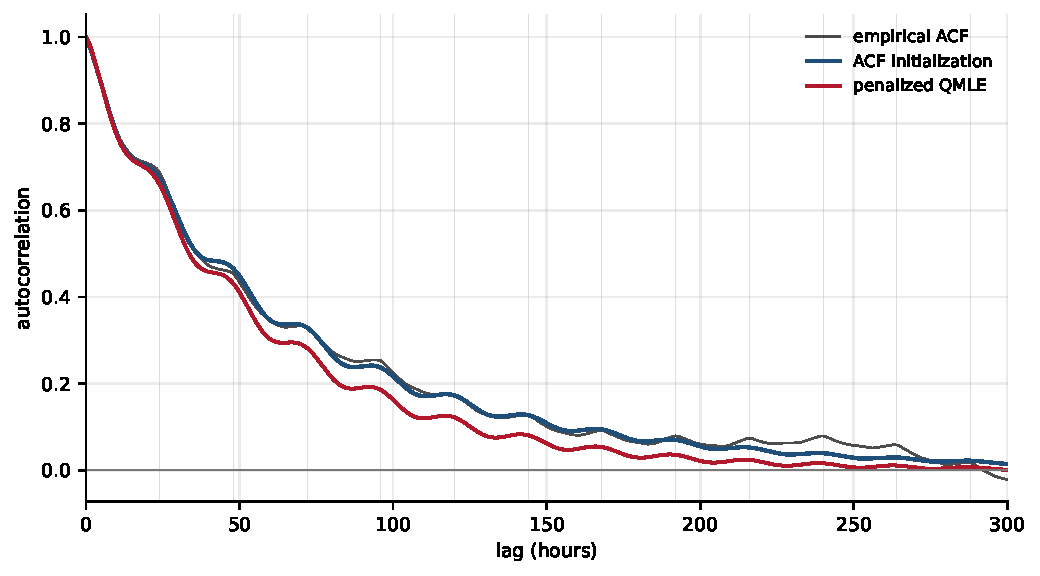
\includegraphics[width=0.78\textwidth]{calibration/temperature_acf_calibration_300.pdf}
  \caption{German temperature ACF calibration over 300 hourly lags, comparing
  the empirical autocorrelation, the multiscale initialization, and the final
  CARMA(4,3) autocorrelation after QMLE.}
  \label{fig:temperature-acf-calibration}
\end{figure}

For temperature, the QMLE step uses \(\lambda_{\mathrm{acf}}=0.1\). This
penalty is lower than for prices because the Gaussian likelihood is on a
different numerical scale. The trade-off is visible in
\cref{fig:temperature-acf-calibration}, where the final ACF is less tightly
matched than in the price calibration. The weaker penalty nevertheless improves the
likelihood fit relative to the ACF initialization, with a final log-likelihood
of \(-22941\), while remaining below the ARMA(4,3) benchmark.

\begin{table}[!htbp]
  \centering
  \caption{Gaussian log-likelihood comparison on the same deseasonalized German
  temperature residuals.}
  \label{tab:temperature-loglik-comparison}
  \begin{tabular}{@{}lr@{}}
    \toprule
    Model & Log-likelihood \\
    \midrule
    CARMA(4,3), ACF initialization & \(-23760\) \\
    CARMA(4,3), QMLE & \(-22941\) \\
    ARMA(1,0) & \(-24612\) \\
    ARMA(4,3) & \(-23173\) \\
    \bottomrule
  \end{tabular}
\end{table}

After QMLE, the slow real half-life is about one and a half days, close to the
solar value and much shorter than the wind and price slow modes. Temperature is
therefore the cleanest two-scale physical marginal, with a fast adjustment, a
one-to-two-day persistence scale, and the fixed daily oscillation.

\begin{figure}[H]
  \centering
  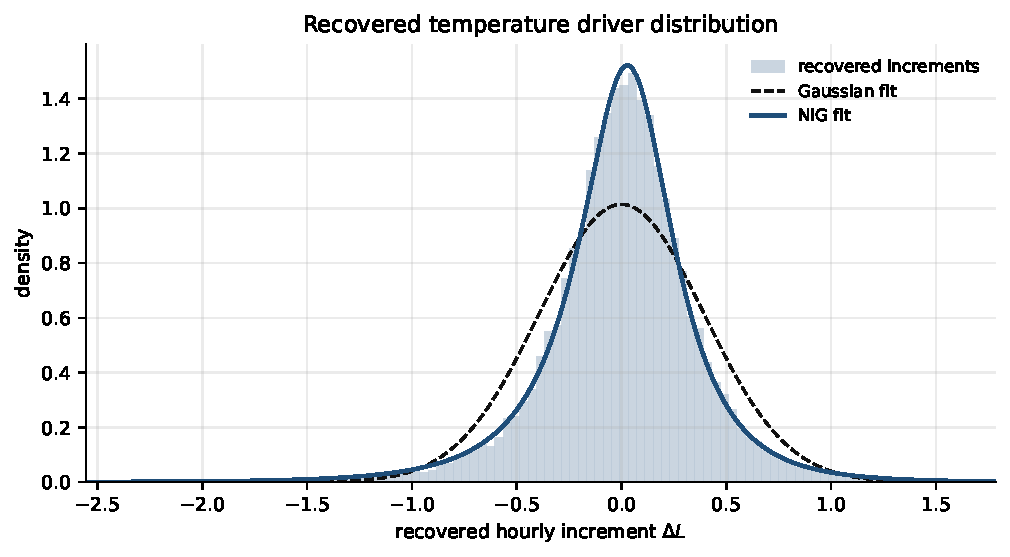
\includegraphics[width=0.78\textwidth]{calibration/temperature_driver_distribution_fit.pdf}
  \caption{Recovered hourly Levy driver increments for the German temperature
  CARMA model. The NIG fit captures the asymmetric and heavy-tailed driver
  distribution better than the Gaussian fit.}
  \label{fig:temperature-driver-distribution}
\end{figure}

\FloatBarrier

\begin{figure}[!htbp]
  \centering
  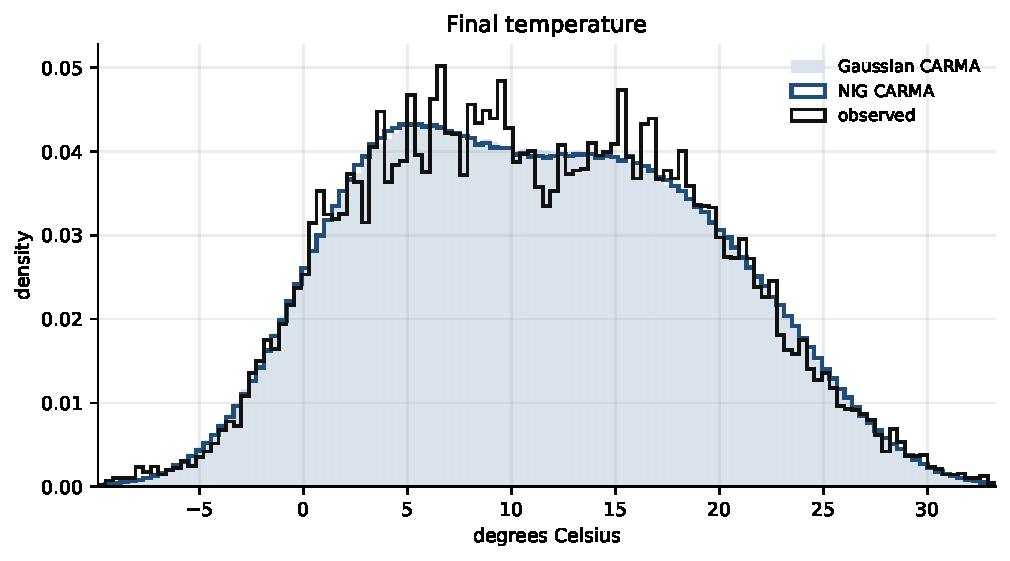
\includegraphics[width=0.74\textwidth]{calibration/temperature_final_distribution.pdf}
  \caption{Distribution check for the final German temperature level, comparing
  the observed data with paths simulated from the Gaussian and NIG CARMA
  marginals.}
  \label{fig:temperature-distribution-checks}
\end{figure}

\FloatBarrier

\subsection{German Solar Production}\label{ssec:german-solar-carma-calibration}

The solar marginal model is fitted to the deseasonalized latent residual
\(\widehat X^Q\) defined after the clear-sky normalization and logit
transformation in \cref{ssec:solar-deseasonalization}. The physical capacity
factor is bounded and has structural nighttime zeros, so the CARMA model is not
applied directly to \(Q_t\). It is estimated in the transformed coordinate, and
simulated paths are mapped back through the inverse clear-sky transformation.

As for temperature, we use a CARMA(4,3) with two real modes and one daily
oscillatory pair. The solar ACF is more specific because it contains periodic
peaks every 24 hours, which must be preserved in calibration. The daily pair is
fixed after the ACF step, while QMLE re-estimates the two real persistence
scales and the moving-average polynomial.

\FloatBarrier

\begin{table}[!htbp]
  \centering
  \caption{German solar CARMA(4,3) half-lives before and after penalized QMLE.}
  \label{tab:solar-carma-half-lives}
  \begin{tabular}{@{}lll@{}}
    \toprule
    Root & Half-life after initialization & Half-life after QMLE \\
    \midrule
    \(\lambda_1\) & \(0.506\) h & \(0.512\) h \\
    \(\lambda_2\) & \(1.74\) d & \(1.57\) d \\
    \(\lambda_o\) & \(2.93\) d & \(2.93\) d \\
    \bottomrule
  \end{tabular}
\end{table}

\FloatBarrier

\begin{figure}[!htbp]
  \centering
  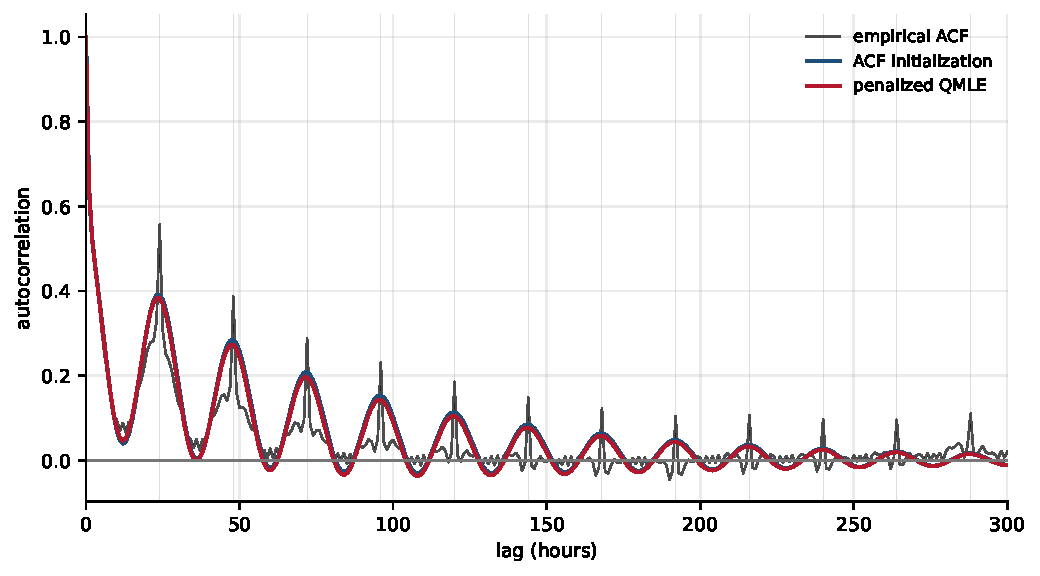
\includegraphics[width=0.78\textwidth]{calibration/solar_acf_calibration_300.pdf}
  \caption{German solar latent-residual ACF calibration over 300 hourly lags,
  comparing the empirical autocorrelation, the multiscale initialization, and
  the final CARMA(4,3) autocorrelation after QMLE.}
  \label{fig:solar-acf-calibration}
\end{figure}

For solar, the QMLE step uses \(\lambda_{\mathrm{acf}}=1000\). This larger
penalty is chosen to preserve the latent ACF structure, in particular its daily
oscillatory component. This choice is also supported by the likelihood
comparison, as the ACF initialization already has a higher log-likelihood than
the ARMA(4,3) benchmark. QMLE then refines the fit only slightly, with a final
log-likelihood of \(-84623\). This leads to only small changes in both the
estimated half-lives and the log-likelihood.

\begin{table}[!htbp]
  \centering
  \caption{Gaussian log-likelihood comparison on the same deseasonalized German
  solar latent residuals.}
  \label{tab:solar-loglik-comparison}
  \begin{tabular}{@{}lr@{}}
    \toprule
    Model & Log-likelihood \\
    \midrule
    CARMA(4,3), ACF initialization & \(-84637\) \\
    CARMA(4,3), QMLE & \(-84623\) \\
    ARMA(1,0) & \(-86462\) \\
    ARMA(4,3) & \(-84786\) \\
    \bottomrule
  \end{tabular}
\end{table}

The solar CARMA(4,3) has roots close to those obtained for temperature. One
real half-life is below one hour, another is around one and a half days, and
the daily oscillations have a damping half-life of about three days.

\begin{figure}[H]
  \centering
  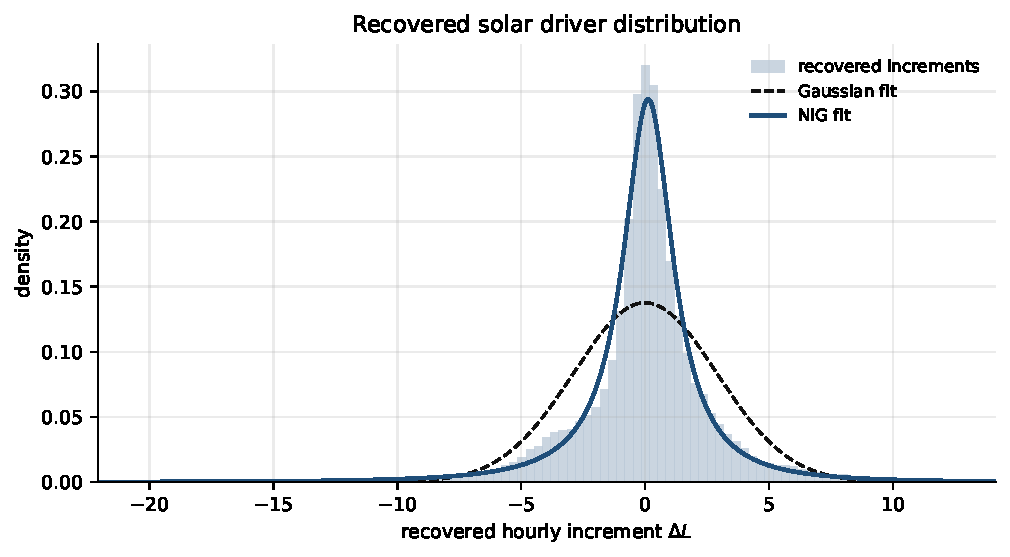
\includegraphics[width=0.78\textwidth]{calibration/solar_driver_distribution_fit.pdf}
  \caption{Recovered hourly Levy driver increments for the German solar CARMA
  model. The NIG fit captures the asymmetric and heavy-tailed driver
  distribution better than the Gaussian fit.}
  \label{fig:solar-driver-distribution}
\end{figure}

\FloatBarrier

\subsection{German Wind Production}\label{ssec:german-wind-carma-calibration}

The wind marginal model is fitted to the deseasonalized logit residual
\(\widehat X^W\) defined in \cref{ssec:wind-deseasonalization}. As for solar,
the CARMA model is estimated in an unconstrained latent coordinate and simulated
paths are mapped back to capacity factors with the inverse logit transform. This
keeps the continuous-time model away from the physical bounds \(0\) and \(1\).

As for temperature and solar, we use a CARMA(4,3) with two real modes and one
daily oscillatory pair. The wind ACF is less tied to a deterministic day-night
structure than solar, but it has longer persistence. The daily pair is fixed
after the ACF step, while QMLE re-estimates the two real persistence scales and
the moving-average polynomial.

\FloatBarrier

\begin{table}[!htbp]
  \centering
  \caption{German wind CARMA(4,3) half-lives before and after penalized QMLE.}
  \label{tab:wind-carma-half-lives}
  \begin{tabular}{@{}lll@{}}
    \toprule
    Root & Half-life after initialization & Half-life after QMLE \\
    \midrule
    \(\lambda_1\) & \(16.1\) h & \(20.9\) h \\
    \(\lambda_o\) & \(3.28\) d & \(3.28\) d \\
    \(\lambda_2\) & \(7.44\) d & \(37.6\) d \\
    \bottomrule
  \end{tabular}
\end{table}

\FloatBarrier

\begin{figure}[!htbp]
  \centering
  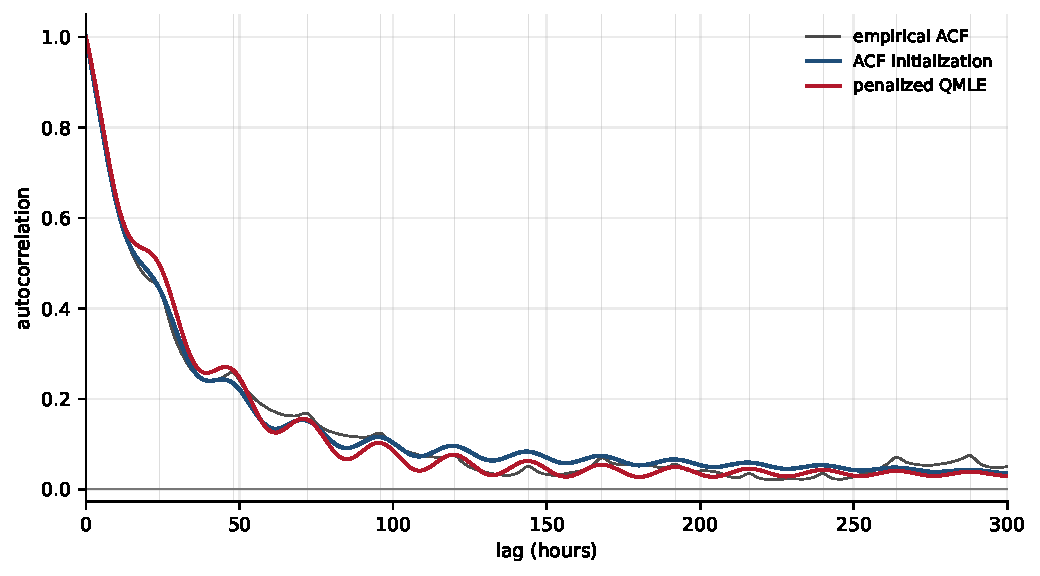
\includegraphics[width=0.78\textwidth]{calibration/wind_acf_calibration_300.pdf}
  \caption{German wind logit-residual ACF calibration over 300 hourly lags,
  comparing the empirical autocorrelation, the multiscale initialization, and
  the final CARMA(4,3) autocorrelation after QMLE.}
  \label{fig:wind-acf-calibration}
\end{figure}

For wind, the QMLE step uses \(\lambda_{\mathrm{acf}}=0.1\), giving a final
log-likelihood of \(-6984\). The fit improves the ACF initialization but
remains below the ARMA(4,3) benchmark in log-likelihood.

\begin{table}[!htbp]
  \centering
  \caption{Gaussian log-likelihood comparison on the same deseasonalized German
  wind logit residuals.}
  \label{tab:wind-loglik-comparison}
  \begin{tabular}{@{}lr@{}}
    \toprule
    Model & Log-likelihood \\
    \midrule
    CARMA(4,3), ACF initialization & \(-7013\) \\
    CARMA(4,3), QMLE & \(-6984\) \\
    ARMA(1,0) & \(-7262\) \\
    ARMA(4,3) & \(-6853\) \\
    \bottomrule
  \end{tabular}
\end{table}

The main difference with solar and temperature is the slow real mode, whose
half-life increases to about 38 days after QMLE. It represents persistent
wind-regime variation in the latent residual.

\begin{figure}[H]
  \centering
  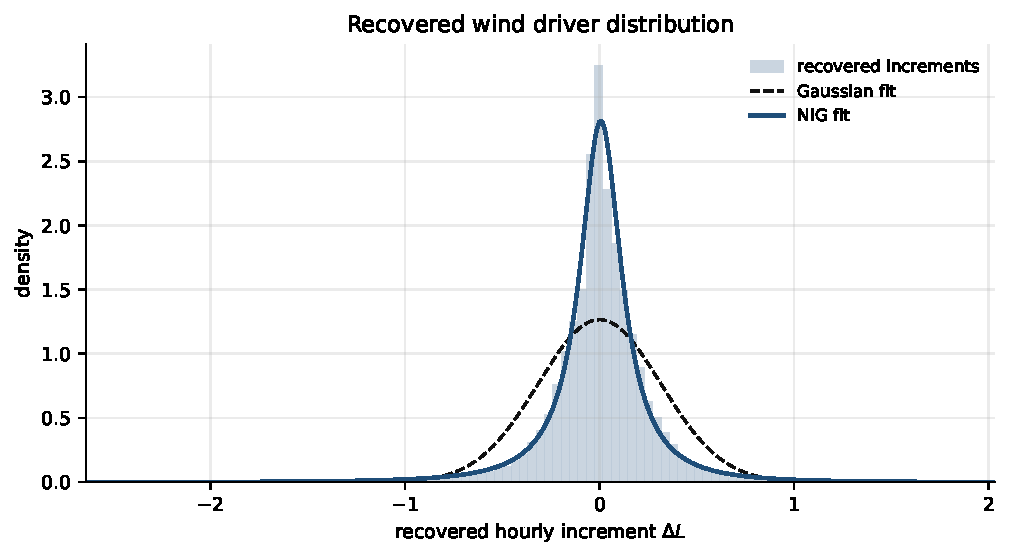
\includegraphics[width=0.78\textwidth]{calibration/wind_driver_distribution_fit.pdf}
  \caption{Recovered hourly Levy driver increments for the German wind CARMA
  model. The NIG fit captures the narrow center and heavy tails better than the
  Gaussian fit.}
  \label{fig:wind-driver-distribution}
\end{figure}

\FloatBarrier

\begin{figure}[!htbp]
  \centering
  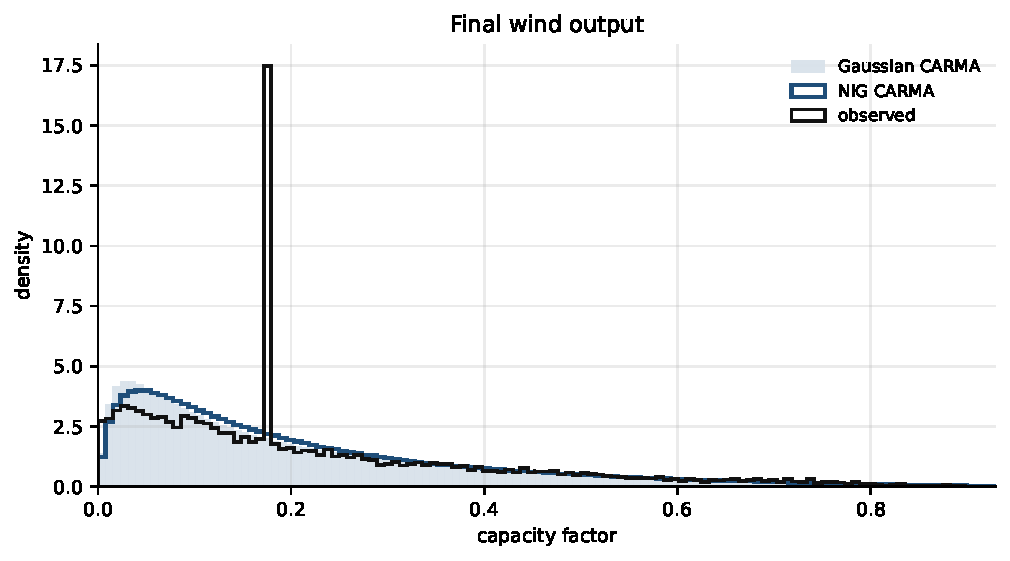
\includegraphics[width=0.74\textwidth]{calibration/wind_final_distribution.pdf}
  \caption{Distribution check for the final German wind capacity factor,
  comparing the observed data with paths simulated from the Gaussian and NIG
  CARMA marginals.}
  \label{fig:wind-distribution-checks}
\end{figure}

\FloatBarrier

\section{Coupling Calibration}\label{sec:coupling-calibration}

\subsection{Coupling Framework}\label{ssec:coupling-framework}

The marginal CARMA models are kept fixed. For a weather or renewable factor
\(F\in\{T,S,W\}\), \(dL^F\) denotes the calibrated marginal driver, with its
variance scale included as in \cref{eq:carma-state-space}. The coupled price
model transmits this factor driver into the price driver.
\begin{align}
  dZ_t^F
  &=
  A_F Z_t^F\,dt+e_F\,dL_t^F,
  &
  Y_t^F &= b_F^\top Z_t^F,
  \nonumber \\
  dZ_t^P
  &=
  A_P Z_t^P\,dt
  +
  e_P\left(\lambda_F\,dL_t^F+dL_t^{P,i}\right),
  &
  Y_t^P &= b_P^\top Z_t^P .
  \label{eq:coupling-state-space}
\end{align}
The parameter \(\lambda_F\) acts only on shocks. It does not change the price
drift, the deterministic seasonality, or the marginal CARMA matrices. If the
factor driver is represented as \(dL_t^F=\sigma_F dW_t^F\) in a Gaussian
covariance calculation, the transmitted shock is equivalently
\(\lambda_F\sigma_F e_P dW_t^F\). The paper uses the \(dL\)-driver convention.

The calibration is not performed on the raw deseasonalized residual levels
\(Y^F\) and \(Y^P\). These correlations are only reported as diagnostics. On
hourly intervals, filtered state-space residuals \(R_i^F\) and \(R_i^P\) are
computed from the fixed marginal filters. If \(dL^F\) is independent of the
idiosyncratic price driver \(dL^{P,i}\), their cross-covariance is proportional
to \(\lambda_F\). Define
\[
  D_{FP}
  =
  \frac{1}{n}\sum_{i=1}^{n}
  (R_i^F-\overline R^F)
  (R_i^P-\overline R^P)^\top
\]
as the empirical cross-covariance, and let \(K_{FP}\) denote the theoretical
cross-covariance generated by the same driver scaling when \(\lambda_F=1\).
The scalar estimate is
\begin{equation}
  \lambda_F
  =
  \frac{b_F^\top D_{FP} b_P}
       {b_F^\top K_{FP} b_P}.
  \label{eq:coupling-lambda-estimator}
\end{equation}
The tables also report the projected state-space residual correlation
\(\mathrm{Corr}(b_P^\top R^P,b_F^\top R^F)\), which is the empirical
correlation associated with the covariance used in
\cref{eq:coupling-lambda-estimator}.
The marginal price driver is then decomposed as
\begin{equation}
  dL_i^{P,m}
  =
  dL_i^{P,i}
  +
  \lambda_F\,dL_i^F,
  \qquad
  dL_i^{P,i}
  =
  dL_i^{P,m}
  -
  \lambda_F\,dL_i^F .
  \label{eq:coupling-driver-decomposition}
\end{equation}
After removing \(\lambda_F dL^F\), the remaining correlation with the factor
driver is used as a direct covariance-level diagnostic for the coupled
simulation model.

\subsection{Temperature--Price Coupling}\label{ssec:temperature-price-coupling}

The raw correlation between the deseasonalized temperature residual and the
deseasonalized German log-price residual is \(-0.24\). A negative sign is
consistent with the winter heating channel, as below-seasonal temperatures tend
to increase electricity demand and spot prices. Since the model acts on shocks,
this level correlation is only a diagnostic.

For temperature, a positive \(dL^T\) is a warmer-than-seasonal shock. A negative
\(\lambda_T\) therefore means that warmer-than-seasonal shocks lower price
shocks, or equivalently that colder-than-seasonal shocks raise price shocks.
This is the expected winter sign, although summer cooling demand can create the
opposite local effect. The pooled estimate is
\[
  \lambda_T = -1.4\times 10^{-3}.
\]

\begin{table}[H]
  \centering
  \caption{Temperature--price coupling diagnostics.}
  \label{tab:temperature-price-coupling-diagnostics}
  \begin{tabular}{@{}lr@{}}
    \toprule
    Quantity & Value \\
    \midrule
    Corr.\((Y^P,Y^T)\) & \(-0.24\) \\
    Corr.\((b_P^\top R^P,b_T^\top R^T)\) & \(-0.040\) \\
    Corr.\((dL^{P,m},dL^T)\) & \(-0.042\) \\
    Corr.\((dL^{P,i},dL^T)\) & \(-9.4{\times}10^{-4}\) \\
    Std.\((\lambda_T dL^T)\) / Std.\((dL^{P,i})\) & \(4.1\%\) \\
    \bottomrule
  \end{tabular}
\end{table}

After removing \(\lambda_T dL^T\), the remaining price driver is close
to uncorrelated with the temperature driver, which supports the covariance
decomposition used for simulation. The ratio in the table is therefore close to
the absolute marginal driver correlation for a simple covariance reason. Let
\(X=dL^{P,m}\), \(Y=dL^{P,i}\), and \(Z=\lambda_T dL^T\). Since \(X=Y+Z\) and
\(\operatorname{Cov}(Y,Z)\simeq 0\) after the removal,
\[
  \operatorname{Cov}(X,Z)
  =
  \operatorname{Cov}(Y+Z,Z)
  \simeq
  \operatorname{Var}(Z).
\]
It follows that \(|\operatorname{Corr}(X,Z)|\simeq \operatorname{Std}(Z)/
\operatorname{Std}(X)\). Since the transmitted component is small,
\(\operatorname{Std}(X)\simeq \operatorname{Std}(Y)\), which gives
\[
  |\operatorname{Corr}(dL^{P,m},dL^T)|
  \simeq
  \frac{\operatorname{Std}(\lambda_T dL^T)}
       {\operatorname{Std}(dL^{P,i})}.
\]

\subsection{Solar--Price Coupling}\label{ssec:solar-price-coupling}

For solar, the raw correlation between the deseasonalized latent residual and
the deseasonalized German log-price residual is \(0.063\). The solar factor is
the deseasonalized clear-sky shortfall variable, so a positive residual
corresponds to a larger latent solar shortfall, not to higher solar production.

Because \(Y^S\) increases with latent solar shortfall, a positive solar shock
represents lower effective solar availability. A positive coupling coefficient
would therefore match the merit-order intuition, as lower solar availability raises
residual demand and price shocks. Unlike temperature and wind, the raw residual
correlation is positive, whereas the projected state-space residual correlation
is negative. The coupling estimator is based on the latter covariance, which
explains the negative sign of the estimate.
\[
  \lambda_S = -8.0\times 10^{-6}.
\]

\begin{table}[H]
  \centering
  \caption{Solar--price coupling diagnostics.}
  \label{tab:solar-price-coupling-diagnostics}
  \begin{tabular}{@{}lr@{}}
    \toprule
    Quantity & Value \\
    \midrule
    Corr.\((Y^P,Y^S)\) & \(0.063\) \\
    Corr.\((b_P^\top R^P,b_S^\top R^S)\) & \(-0.0018\) \\
    Corr.\((dL^{P,m},dL^S)\) & \(-1.0{\times}10^{-3}\) \\
    Corr.\((dL^{P,i},dL^S)\) & \(7.8{\times}10^{-4}\) \\
    Std.\((\lambda_S dL^S)\) / Std.\((dL^{P,i})\) & \(0.18\%\) \\
    \bottomrule
  \end{tabular}
\end{table}

The solar driver correlation and the transmitted-shock standard-deviation ratio
are both close to zero. Solar has the smallest ratio among the three factors,
which questions the relevance of a coupled price--solar shock model for this
dataset.

\subsection{Wind--Price Coupling}\label{ssec:wind-price-coupling}

For wind, the raw correlation between the logit residual and the German
log-price residual is \(-0.50\). The wind transform is monotone in the capacity
factor, so a positive wind residual corresponds to above-seasonal wind
production. The negative sign is consistent with the merit-order effect.

For wind, a positive \(dL^W\) is an above-seasonal production shock. The expected
coupling sign is therefore negative, since higher wind production lowers
residual demand. The estimate is
\[
  \lambda_W = -1.7\times 10^{-3}.
\]

\begin{table}[H]
  \centering
  \caption{Wind--price coupling diagnostics.}
  \label{tab:wind-price-coupling-diagnostics}
  \begin{tabular}{@{}lr@{}}
    \toprule
    Quantity & Value \\
    \midrule
    Corr.\((Y^P,Y^W)\) & \(-0.50\) \\
    Corr.\((b_P^\top R^P,b_W^\top R^W)\) & \(-0.040\) \\
    Corr.\((dL^{P,m},dL^W)\) & \(-0.040\) \\
    Corr.\((dL^{P,i},dL^W)\) & \(3.7{\times}10^{-5}\) \\
    Std.\((\lambda_W dL^W)\) / Std.\((dL^{P,i})\) & \(4.0\%\) \\
    \bottomrule
  \end{tabular}
\end{table}

The wind channel is the clearest renewable coupling in this calibration. The
marginal price driver has a small negative wind correlation, and after removing
\(\lambda_W dL^W\) the remaining idiosyncratic driver has no detectable
linear correlation with wind. The transmitted component remains small, with a
standard-deviation ratio close to the temperature one, and this ratio is
consistent with the state-space residual correlation.

\FloatBarrier

\section{Conclusion}\label{sec:conclusion}

The calibration procedure used in this paper provides accurate continuous-time
CARMA marginals for prices, temperature, solar production and wind production.
The ACF initialization gives interpretable persistence scales, while the QMLE
step improves the likelihood without losing the main autocorrelation structure.
Compared with discrete ARMA benchmarks, the CARMA specification keeps a
continuous-time state-space representation that is directly usable for joint
simulation.

For the coupled model, the relevant dependence is measured at the state-space
and driver level rather than on raw residual levels. Temperature and wind
transmit small but visible shocks to the price driver, with standard-deviation
ratios around \(4\%\), while the solar coupling is much weaker. This questions
the relevance of a linear coupled price--solar shock model on this dataset. More
generally, the present framework lets physical factors affect prices only
through shocks. Allowing temperature, wind or solar to also enter the price
drift could capture slower structural effects, and a multivariate CARMA
specification is a natural direction for such an extension.


\clearpage
\appendix
\numberwithin{figure}{section}
\numberwithin{table}{section}
\section*{Appendix}
The appendix reports supplementary graphical and numerical diagnostics. It is
organized into data and deseasonalization checks, marginal CARMA calibration
outputs, and residual scatter plots for the coupling calibration.

\section{Data and Deseasonalization Diagnostics}
\label{app:data-deseasonalization}

This section reports additional preprocessing diagnostics. Weekly plots use
1--8 June 2025, while the price daily factor is shown over the first semester of
2025.

\subsection{Electricity Prices}
\label{app:price-deseasonalization}

\begin{figure}[!htbp]
  \centering
  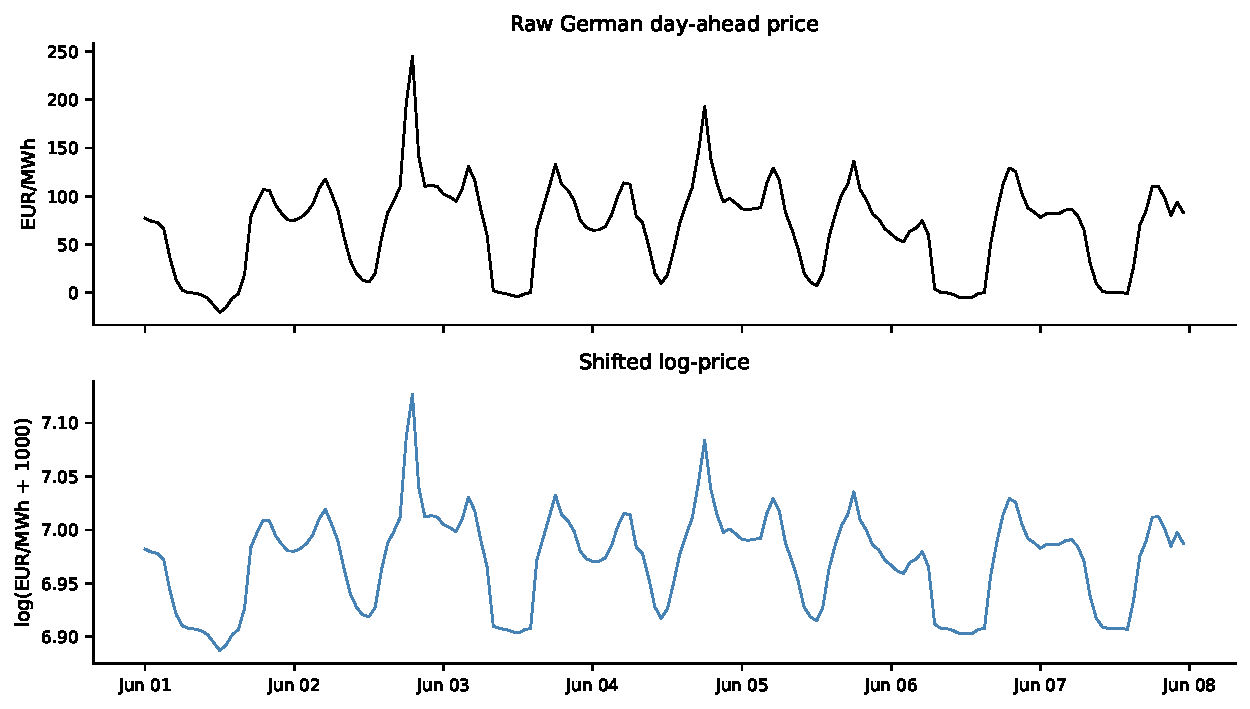
\includegraphics[width=0.92\textwidth]{appendix/price_raw_and_shifted_log_week.pdf}
  \caption{German day-ahead price and shifted log-price over the common
  appendix week. The shift makes the logarithmic coordinate well-defined when
  hourly prices are negative.}
  \label{fig:app-price-raw-log-week}
\end{figure}

\begin{figure}[!htbp]
  \centering
  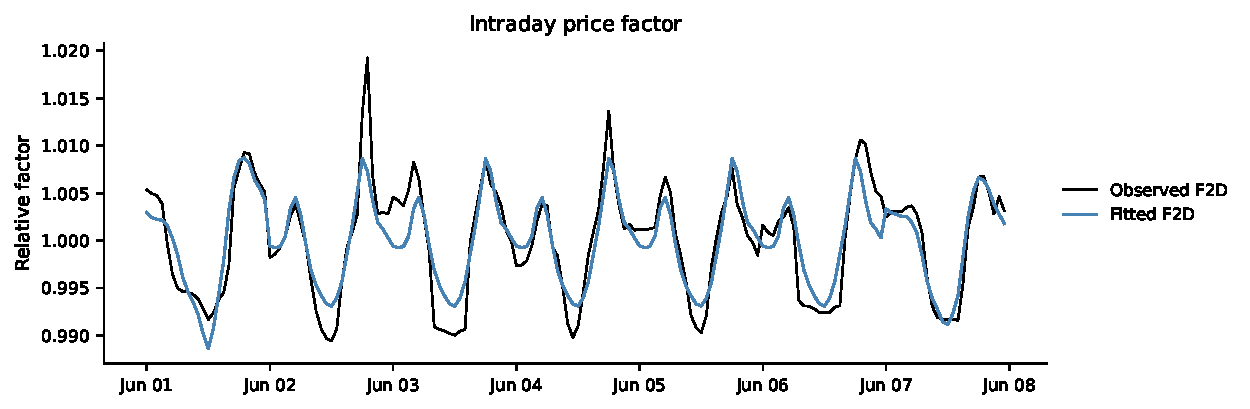
\includegraphics[width=0.88\textwidth]{appendix/price_f2d_week.pdf}
  \caption{Observed and fitted intraday price factor over the common appendix
  week. The observed factor is the shifted log-price divided by its daily mean.}
  \label{fig:app-price-f2d-week}
\end{figure}

\begin{figure}[!htbp]
  \centering
  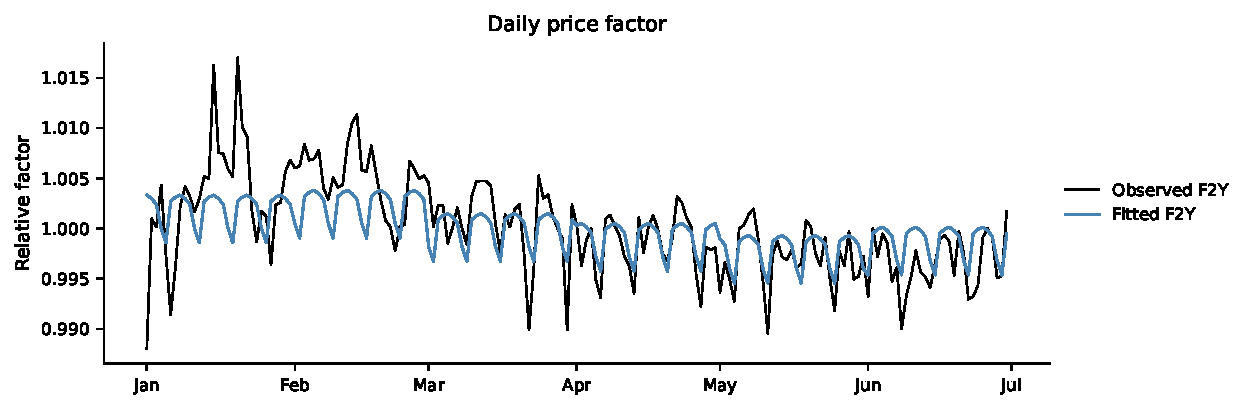
\includegraphics[width=0.88\textwidth]{appendix/price_f2y_first_semester.pdf}
  \caption{Observed and fitted daily price factor over the first semester of
  2025. The observed factor is the daily mean shifted log-price divided by its
  yearly mean.}
  \label{fig:app-price-f2y-semester}
\end{figure}

\begin{figure}[!htbp]
  \centering
  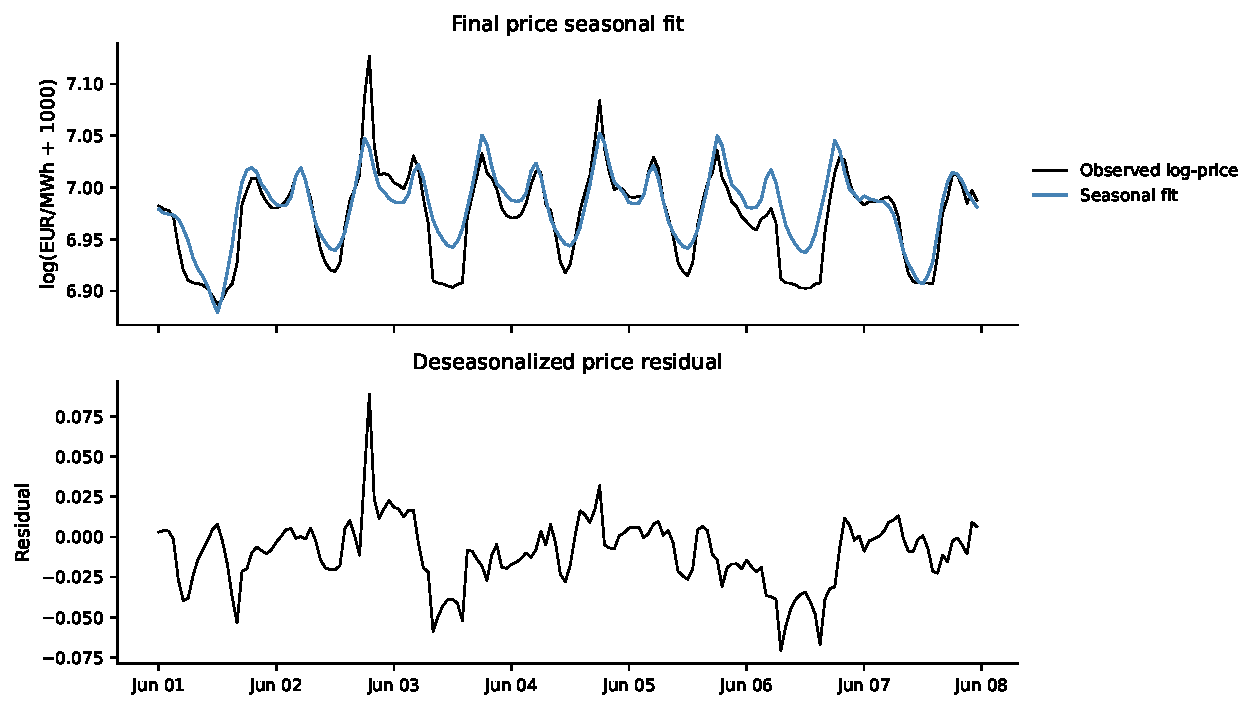
\includegraphics[width=0.92\textwidth]{appendix/price_final_fit_and_residual_week.pdf}
  \caption{Final deterministic price seasonality and resulting deseasonalized
  log-price residual over the common appendix week.}
  \label{fig:app-price-final-fit-week}
\end{figure}

\begin{figure}[!htbp]
  \centering
  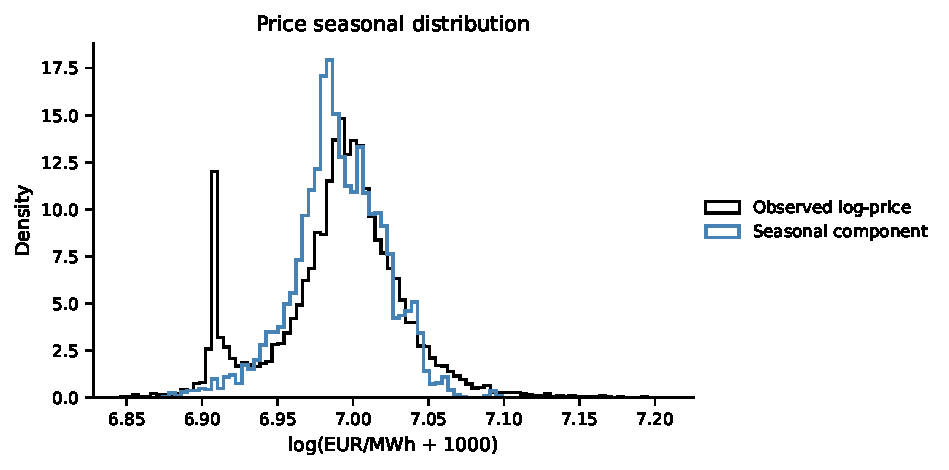
\includegraphics[width=0.72\textwidth]{appendix/price_log_distribution.pdf}
  \caption{Marginal distribution of the shifted log-price and of its fitted
  deterministic seasonal component over the 2023--2025 calibration sample.}
  \label{fig:app-price-log-distribution}
\end{figure}

\FloatBarrier

\clearpage
\subsection{Temperature}
\label{app:temperature-deseasonalization}

\begin{figure}[!htbp]
  \centering
  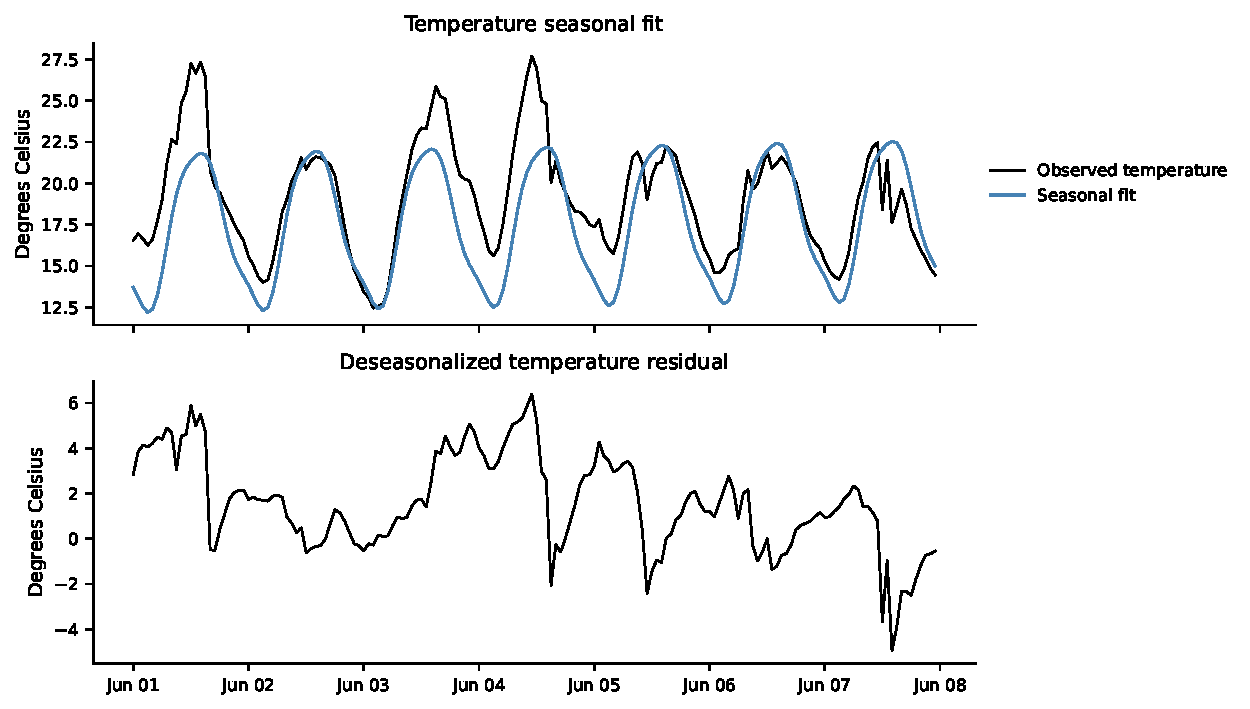
\includegraphics[width=0.92\textwidth]{appendix/temperature_fit_and_residual_week.pdf}
  \caption{Temperature seasonal fit and resulting deseasonalized residual over
  the common appendix week.}
  \label{fig:app-temperature-fit-week}
\end{figure}

\begin{figure}[!htbp]
  \centering
  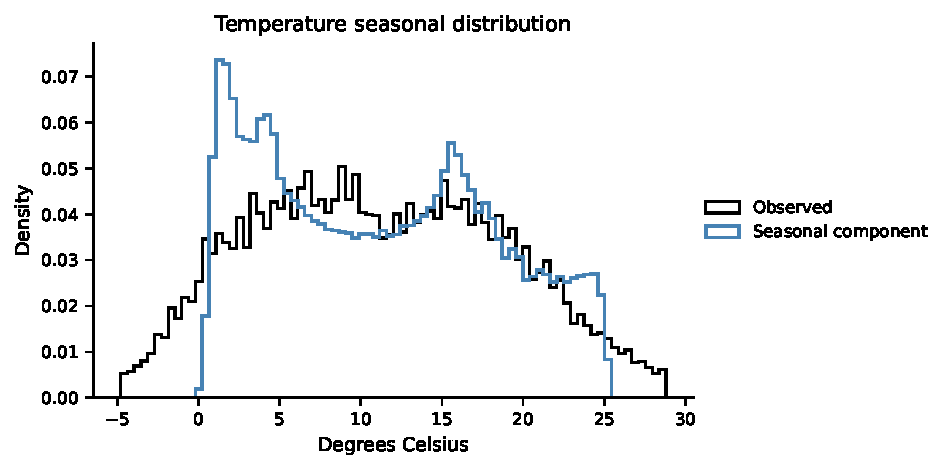
\includegraphics[width=0.72\textwidth]{appendix/temperature_distribution.pdf}
  \caption{Marginal distribution of observed temperature and of the fitted
  deterministic seasonal component over the 2023--2025 calibration sample.}
  \label{fig:app-temperature-distribution}
\end{figure}

\FloatBarrier

\clearpage
\subsection{Solar Capacity Factors}
\label{app:solar-deseasonalization}

\begin{figure}[!htbp]
  \centering
  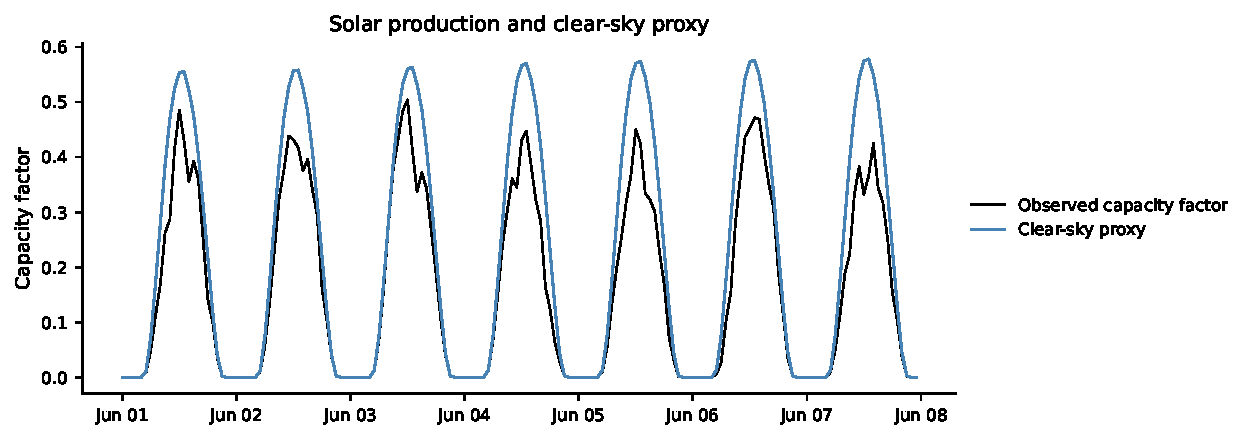
\includegraphics[width=0.88\textwidth]{appendix/solar_clear_sky_week.pdf}
  \caption{Observed solar capacity factor and clear-sky proxy over the common
  appendix week. The clear-sky proxy is the deterministic envelope used before
  constructing the latent logit coordinate.}
  \label{fig:app-solar-clear-sky-week}
\end{figure}

\begin{figure}[!htbp]
  \centering
  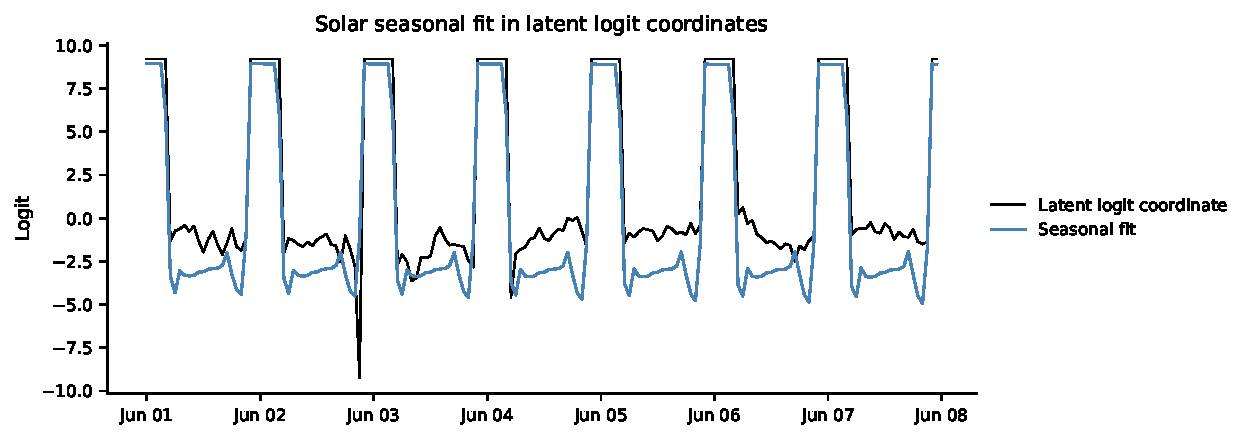
\includegraphics[width=0.88\textwidth]{appendix/solar_logit_fit_week.pdf}
  \caption{Solar seasonal fit in the latent logit coordinate over the common
  appendix week. This is the coordinate in which the deterministic seasonality
  is estimated.}
  \label{fig:app-solar-logit-fit-week}
\end{figure}

\begin{figure}[!htbp]
  \centering
  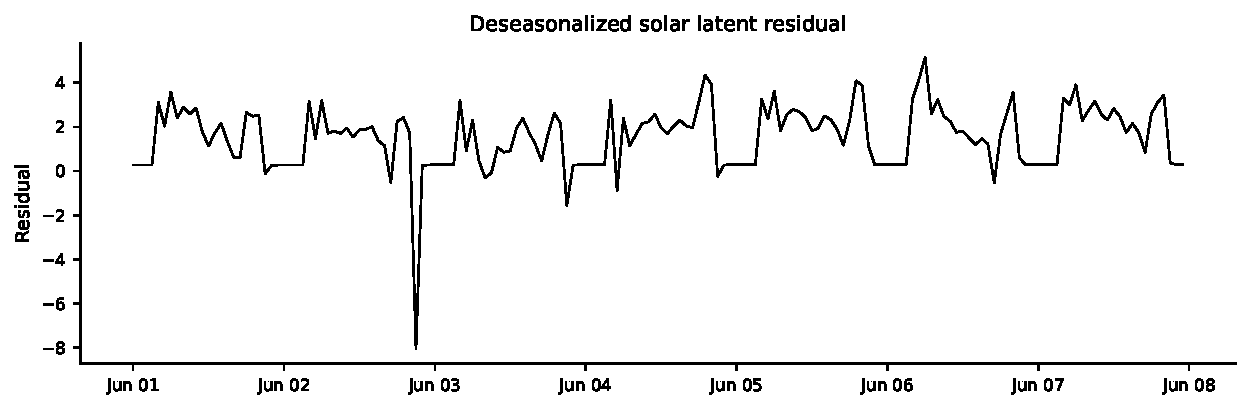
\includegraphics[width=0.88\textwidth]{appendix/solar_logit_residual_week.pdf}
  \caption{Deseasonalized solar residual in the latent logit coordinate over the
  common appendix week. This residual is the stochastic component calibrated
  with a CARMA model.}
  \label{fig:app-solar-logit-residual-week}
\end{figure}

\clearpage
\begin{figure}[!htbp]
  \centering
  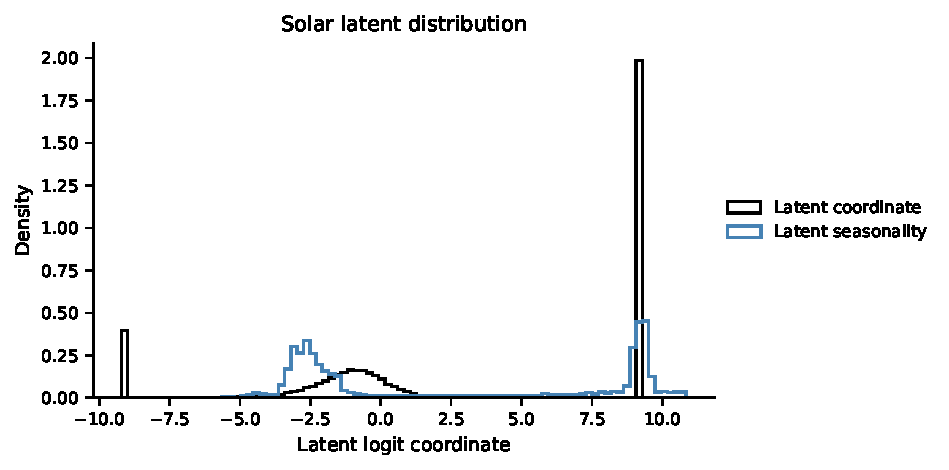
\includegraphics[width=0.72\textwidth]{appendix/solar_latent_distribution.pdf}
  \caption{Marginal distribution of the solar latent coordinate and of its
  fitted deterministic seasonal component over the calibration sample.}
  \label{fig:app-solar-latent-distribution}
\end{figure}

\FloatBarrier

\clearpage
\subsection{Wind Capacity Factors}
\label{app:wind-deseasonalization}

\begin{figure}[!htbp]
  \centering
  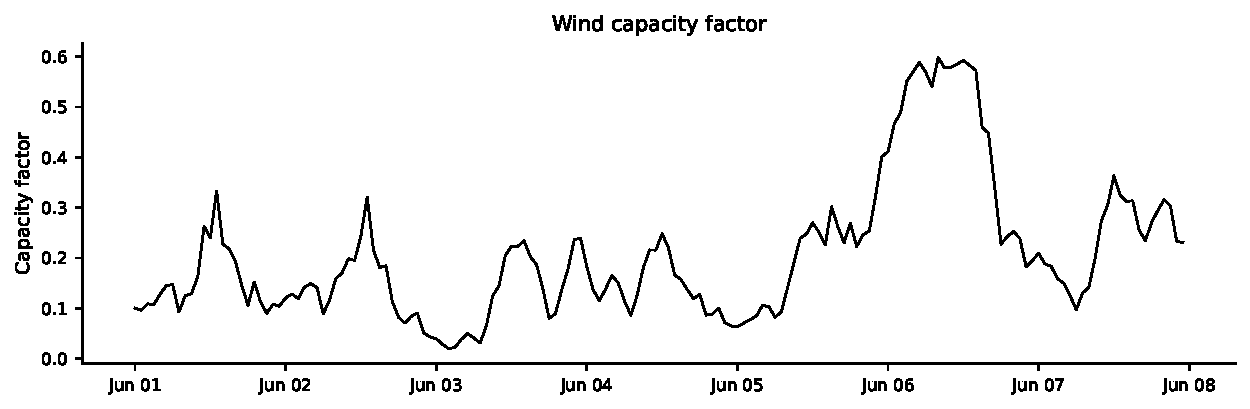
\includegraphics[width=0.88\textwidth]{appendix/wind_capacity_factor_week.pdf}
  \caption{Observed wind capacity factor over the common appendix week.}
  \label{fig:app-wind-capacity-factor-week}
\end{figure}

\begin{figure}[!htbp]
  \centering
  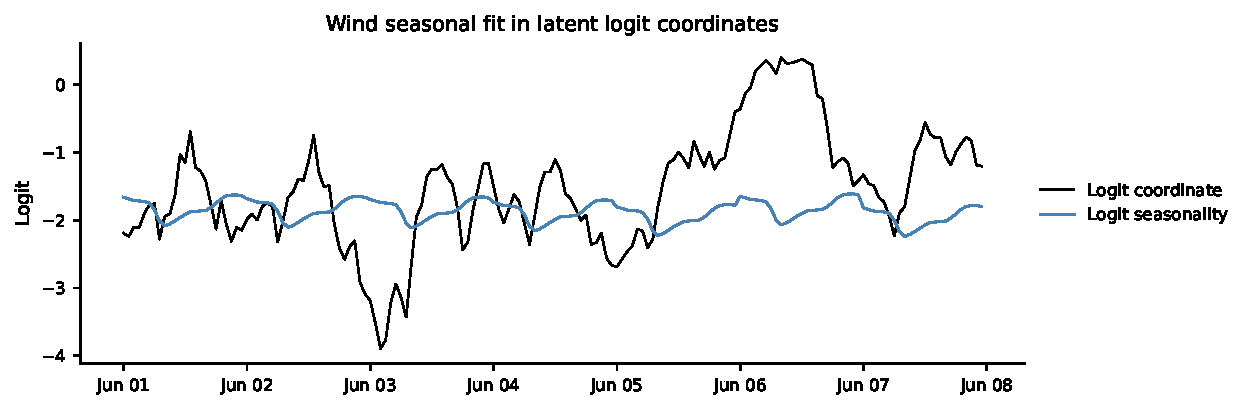
\includegraphics[width=0.88\textwidth]{appendix/wind_logit_fit_week.pdf}
  \caption{Wind seasonal fit in the latent logit coordinate over the common
  appendix week. This is the coordinate in which the deterministic seasonality
  is estimated.}
  \label{fig:app-wind-logit-fit-week}
\end{figure}

\begin{figure}[!htbp]
  \centering
  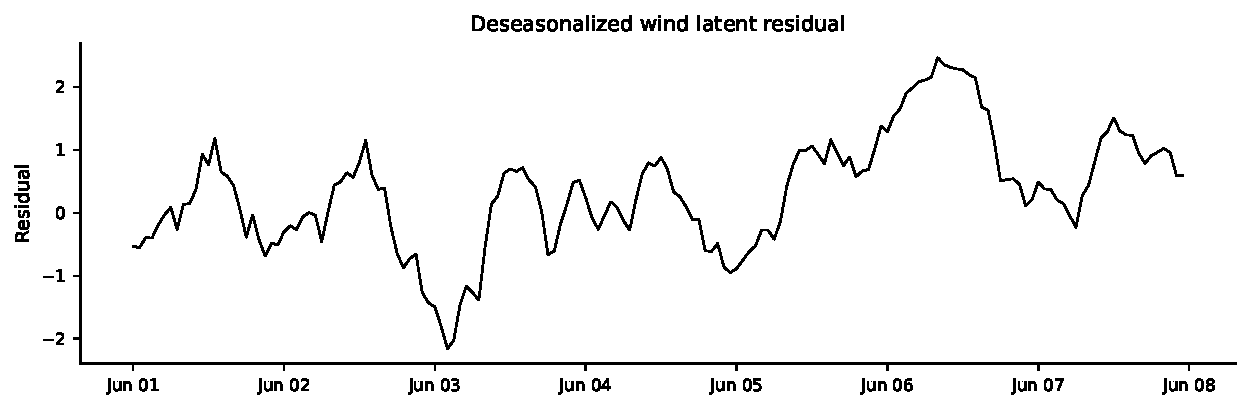
\includegraphics[width=0.88\textwidth]{appendix/wind_logit_residual_week.pdf}
  \caption{Deseasonalized wind residual in the latent logit coordinate over the
  common appendix week. This residual is the stochastic component calibrated
  with a CARMA model.}
  \label{fig:app-wind-logit-residual-week}
\end{figure}

\clearpage
\begin{figure}[!htbp]
  \centering
  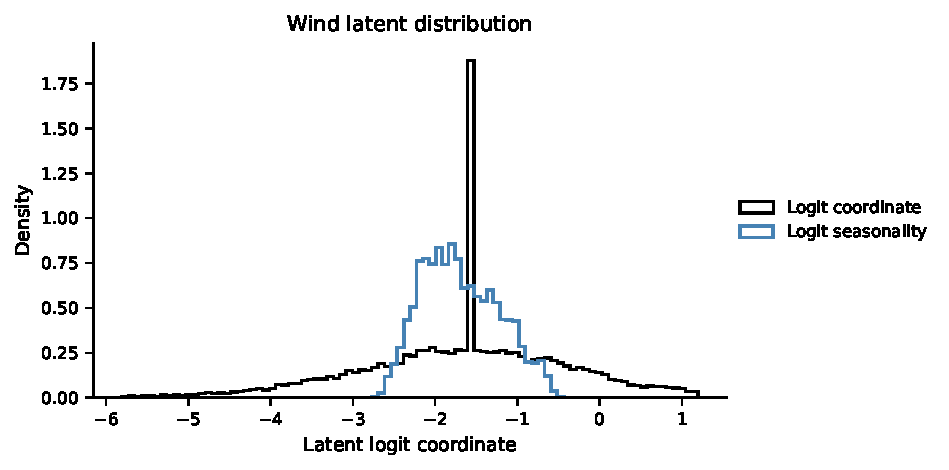
\includegraphics[width=0.72\textwidth]{appendix/wind_latent_distribution.pdf}
  \caption{Marginal distribution of the wind latent logit coordinate and of its
  fitted deterministic seasonal component over the calibration sample.}
  \label{fig:app-wind-latent-distribution}
\end{figure}

\FloatBarrier

\clearpage
\section{Marginal Calibration Diagnostics}

\label{app:marginal-calibration}



\subsection{German Spot Prices}

\label{app:price-calibration}

\begin{table}[H]
  \centering
  \caption{Full German spot price CARMA(5,4) calibration parameters.}
  \label{tab:app-price-carma-params}
  \small
  \begin{tabular}{@{}lll@{}}
    \toprule
    Quantity & ACF initialization & QMLE \\
    \midrule
    Log-likelihood & \(77562\) & \(77709\) \\
    Levy drift \(m\) & \(1.40{\times}10^{-5}\) & \(8.47{\times}10^{-6}\) \\
    Levy variance \(\nu^2\) & \(1.88{\times}10^{-4}\) & \(1.75{\times}10^{-4}\) \\
    \midrule
    \(\lambda_1\) & \(-0.263\) & \(-0.153\) \\
    \(\lambda_2\) & \(-0.0242\) & \(-0.0193\) \\
    \(\lambda_3\) & \(-2.41{\times}10^{-4}\) & \(-3.51{\times}10^{-4}\) \\
    \(\lambda_o\) & \(-0.00400\pm0.262i\) & \(-0.00400\pm0.262i\) \\
    \midrule
    \(a_1\) & \(0.296\) & \(0.181\) \\
    \(a_2\) & \(0.0773\) & \(0.0730\) \\
    \(a_3\) & \(0.0198\) & \(0.0119\) \\
    \(a_4\) & \(4.41{\times}10^{-4}\) & \(2.07{\times}10^{-4}\) \\
    \(a_5\) & \(1.05{\times}10^{-7}\) & \(7.11{\times}10^{-8}\) \\
    \midrule
    \(b_0\) & \(7.84{\times}10^{-6}\) & \(4.89{\times}10^{-6}\) \\
    \(b_1\) & \(0.00719\) & \(0.00387\) \\
    \(b_2\) & \(0.0713\) & \(0.0672\) \\
    \(b_3\) & \(0.130\) & \(0.0809\) \\
    \(b_4\) & \(1.00\) & \(1.00\) \\
    \bottomrule
  \end{tabular}
\end{table}



\begin{table}[H]
  \centering
  \caption{NIG fit for recovered hourly Levy increments in the German spot price model.}
  \label{tab:app-price-nig-params}
  \small
  \begin{tabular}{@{}lr@{}}
    \toprule
    Quantity & Value \\
    \midrule
    \(\alpha\) & \(47.5\) \\
    \(\beta\) & \(-5.07\) \\
    \(\delta\) & \(0.00687\) \\
    \(\mu\) & \(7.40{\times}10^{-4}\) \\
    \(\gamma\) & \(47.2\) \\
    Mean & \(1.89{\times}10^{-6}\) \\
    Standard deviation & \(0.0121\) \\
    Skewness & \(-0.563\) \\
    Excess kurtosis & \(9.68\) \\
    Log-likelihood & \(83442\) \\
    \bottomrule
  \end{tabular}
\end{table}



\begin{figure}[H]
  \centering
  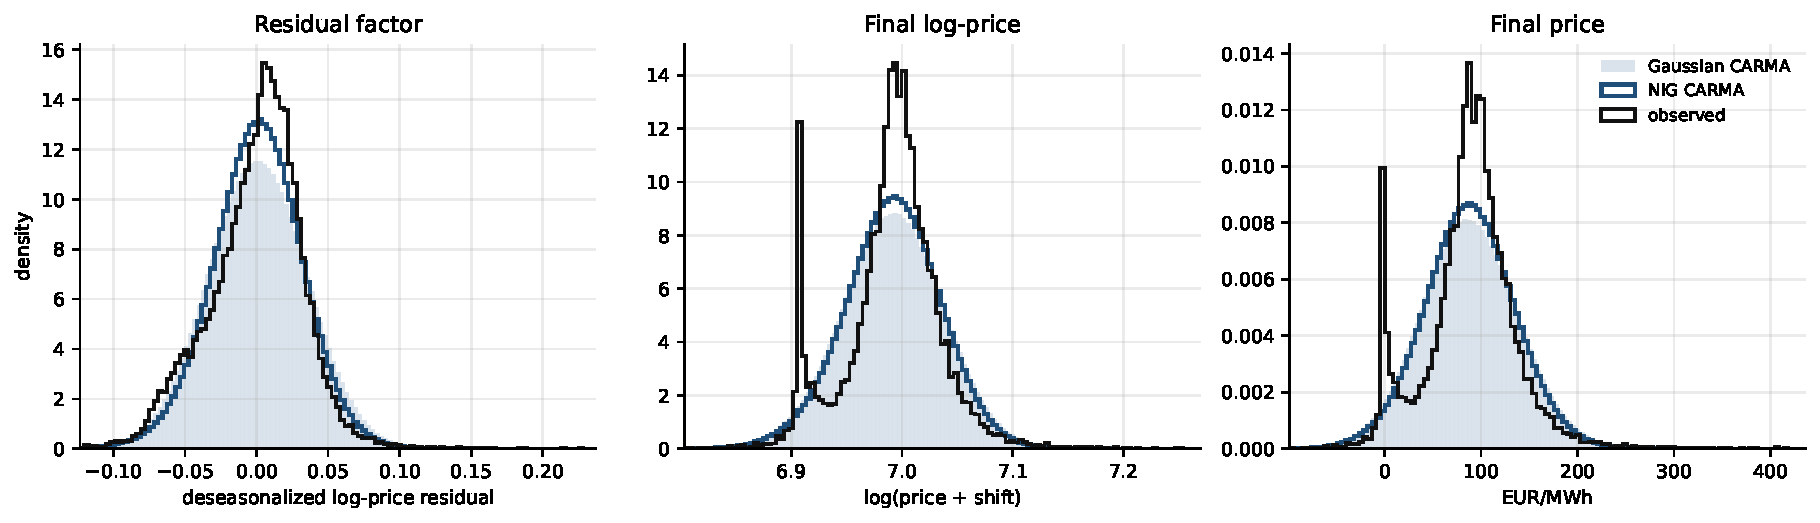
\includegraphics[width=0.82\textwidth]{calibration/price_spot_distribution_checks.pdf}
  \caption{Distribution checks for the German price marginal model at the residual factor, shifted log-price, and EUR/MWh price levels.}
  \label{fig:app-price-distribution-checks}
\end{figure}



\FloatBarrier

\clearpage



\subsection{Temperature}

\label{app:temperature-calibration}

\begin{table}[H]
  \centering
  \caption{Full temperature CARMA(4,3) calibration parameters.}
  \label{tab:app-temperature-carma-params}
  \small
  \begin{tabular}{@{}lll@{}}
    \toprule
    Quantity & ACF initialization & QMLE \\
    \midrule
    Log-likelihood & \(-23760\) & \(-22941\) \\
    Levy drift \(m\) & \(5.48{\times}10^{-4}\) & \(2.85{\times}10^{-4}\) \\
    Levy variance \(\nu^2\) & \(0.350\) & \(0.161\) \\
    \midrule
    \(\lambda_1\) & \(-0.0272\) & \(-1.31\) \\
    \(\lambda_2\) & \(-0.0119\) & \(-0.0182\) \\
    \(\lambda_o\) & \(-0.00953\pm0.262i\) & \(-0.00953\pm0.262i\) \\
    \midrule
    \(a_1\) & \(0.0582\) & \(1.35\) \\
    \(a_2\) & \(0.0697\) & \(0.118\) \\
    \(a_3\) & \(0.00269\) & \(0.0915\) \\
    \(a_4\) & \(2.23{\times}10^{-5}\) & \(0.00163\) \\
    \midrule
    \(b_0\) & \(0.00136\) & \(0.163\) \\
    \(b_1\) & \(0.0690\) & \(0.201\) \\
    \(b_2\) & \(0.0782\) & \(2.57\) \\
    \(b_3\) & \(1.00\) & \(1.00\) \\
    \bottomrule
  \end{tabular}
\end{table}



\begin{table}[H]
  \centering
  \caption{NIG fit for recovered hourly Levy increments in the temperature model.}
  \label{tab:app-temperature-nig-params}
  \small
  \begin{tabular}{@{}lr@{}}
    \toprule
    Quantity & Value \\
    \midrule
    \(\alpha\) & \(2.06\) \\
    \(\beta\) & \(-0.257\) \\
    \(\delta\) & \(0.299\) \\
    \(\mu\) & \(0.0372\) \\
    \(\gamma\) & \(2.05\) \\
    Mean & \(-2.58{\times}10^{-4}\) \\
    Standard deviation & \(0.385\) \\
    Skewness & \(-0.477\) \\
    Excess kurtosis & \(5.20\) \\
    Log-likelihood & \(-9716\) \\
    \bottomrule
  \end{tabular}
\end{table}



\begin{figure}[H]
  \centering
  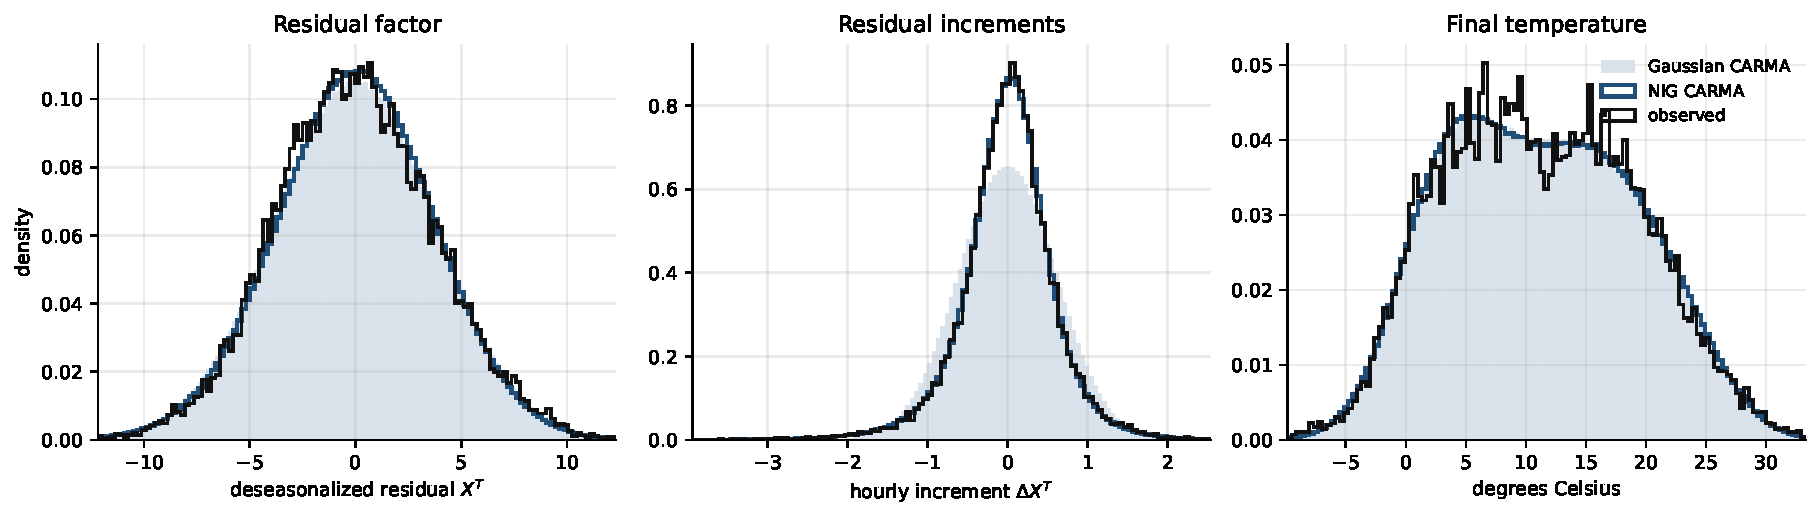
\includegraphics[width=0.97\textwidth]{calibration/temperature_distribution_checks.pdf}
  \caption{Distribution checks for the German temperature marginal model at the deseasonalized residual, hourly residual-increment, and physical temperature levels.}
  \label{fig:app-temperature-distribution-checks}
\end{figure}



\FloatBarrier

\clearpage



\subsection{Solar Capacity Factor}

\label{app:solar-calibration}

\begin{table}[H]
  \centering
  \caption{Full solar capacity factor CARMA(4,3) calibration parameters.}
  \label{tab:app-solar-carma-params}
  \small
  \begin{tabular}{@{}lll@{}}
    \toprule
    Quantity & ACF initialization & QMLE \\
    \midrule
    Log-likelihood & \(-84637\) & \(-84623\) \\
    Levy drift \(m\) & \(1.14{\times}10^{-4}\) & \(1.27{\times}10^{-4}\) \\
    Levy variance \(\nu^2\) & \(9.27\) & \(9.12\) \\
    \midrule
    \(\lambda_1\) & \(-1.37\) & \(-1.35\) \\
    \(\lambda_2\) & \(-0.0166\) & \(-0.0184\) \\
    \(\lambda_o\) & \(-0.00984\pm0.262i\) & \(-0.00984\pm0.262i\) \\
    \midrule
    \(a_1\) & \(1.41\) & \(1.39\) \\
    \(a_2\) & \(0.119\) & \(0.121\) \\
    \(a_3\) & \(0.0957\) & \(0.0947\) \\
    \(a_4\) & \(0.00156\) & \(0.00171\) \\
    \midrule
    \(b_0\) & \(0.00848\) & \(0.00899\) \\
    \(b_1\) & \(0.0836\) & \(0.0819\) \\
    \(b_2\) & \(0.231\) & \(0.239\) \\
    \(b_3\) & \(1.00\) & \(1.00\) \\
    \bottomrule
  \end{tabular}
\end{table}



\begin{table}[H]
  \centering
  \caption{NIG fit for recovered hourly Levy increments in the solar capacity factor model.}
  \label{tab:app-solar-nig-params}
  \small
  \begin{tabular}{@{}lr@{}}
    \toprule
    Quantity & Value \\
    \midrule
    \(\alpha\) & \(0.136\) \\
    \(\beta\) & \(-0.0149\) \\
    \(\delta\) & \(1.24\) \\
    \(\mu\) & \(0.136\) \\
    \(\gamma\) & \(0.135\) \\
    Mean & \(1.33{\times}10^{-4}\) \\
    Standard deviation & \(3.04\) \\
    Skewness & \(-0.803\) \\
    Excess kurtosis & \(18.8\) \\
    Log-likelihood & \(-91910\) \\
    \bottomrule
  \end{tabular}
\end{table}



\begin{figure}[H]
  \centering
  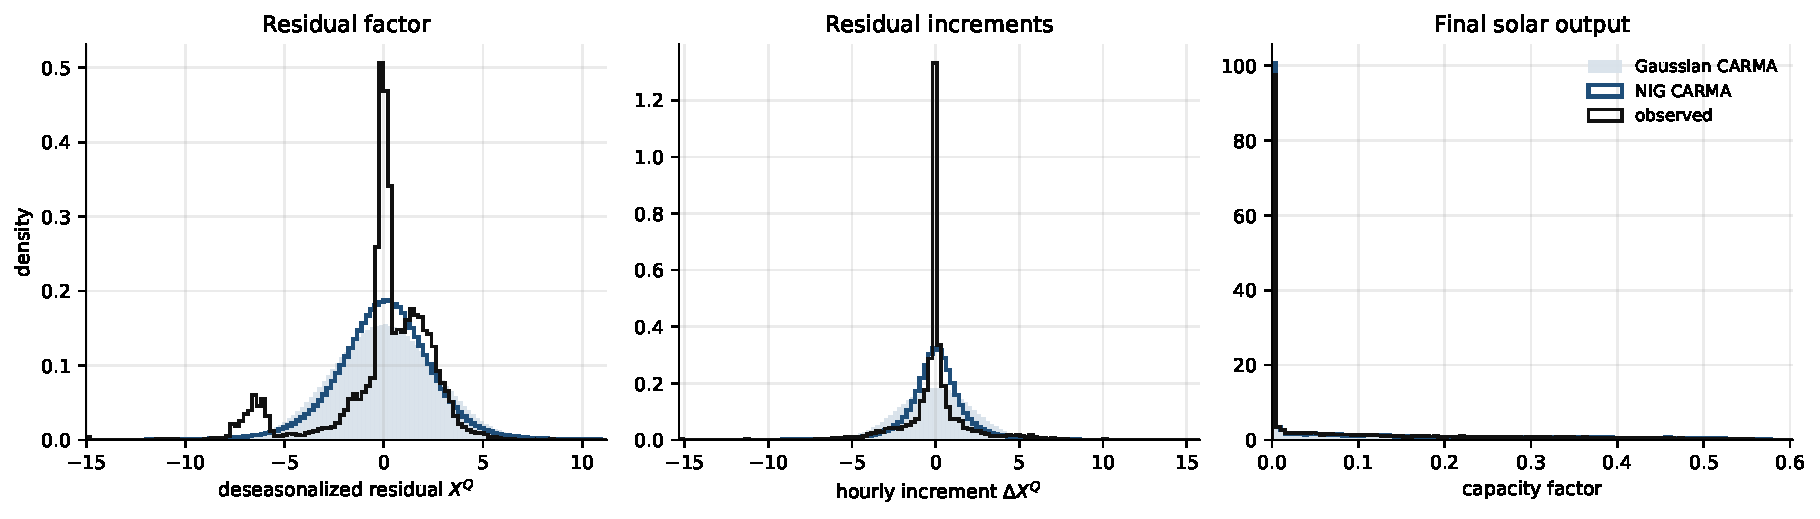
\includegraphics[width=0.97\textwidth]{calibration/solar_distribution_checks.pdf}
  \caption{Distribution checks for the German solar marginal model at the deseasonalized latent residual, hourly residual-increment, and physical capacity-factor levels.}
  \label{fig:app-solar-distribution-checks}
\end{figure}



\FloatBarrier

\clearpage



\subsection{Wind Capacity Factor}

\label{app:wind-calibration}

\begin{table}[H]
  \centering
  \caption{Full wind capacity factor CARMA(4,3) calibration parameters.}
  \label{tab:app-wind-carma-params}
  \small
  \begin{tabular}{@{}lll@{}}
    \toprule
    Quantity & ACF initialization & QMLE \\
    \midrule
    Log-likelihood & \(-7013\) & \(-6984\) \\
    Levy drift \(m\) & \(6.36{\times}10^{-5}\) & \(1.57{\times}10^{-5}\) \\
    Levy variance \(\nu^2\) & \(0.102\) & \(0.0993\) \\
    \midrule
    \(\lambda_1\) & \(-0.0431\) & \(-0.0331\) \\
    \(\lambda_2\) & \(-0.00388\) & \(-7.68{\times}10^{-4}\) \\
    \(\lambda_o\) & \(-0.00880\pm0.262i\) & \(-0.00880\pm0.262i\) \\
    \midrule
    \(a_1\) & \(0.0646\) & \(0.0515\) \\
    \(a_2\) & \(0.0696\) & \(0.0692\) \\
    \(a_3\) & \(0.00323\) & \(0.00233\) \\
    \(a_4\) & \(1.15{\times}10^{-5}\) & \(1.75{\times}10^{-6}\) \\
    \midrule
    \(b_0\) & \(4.27{\times}10^{-4}\) & \(9.23{\times}10^{-5}\) \\
    \(b_1\) & \(0.0685\) & \(0.0689\) \\
    \(b_2\) & \(0.0472\) & \(0.0539\) \\
    \(b_3\) & \(1.00\) & \(1.00\) \\
    \bottomrule
  \end{tabular}
\end{table}



\begin{table}[H]
  \centering
  \caption{NIG fit for recovered hourly Levy increments in the wind capacity factor model.}
  \label{tab:app-wind-nig-params}
  \small
  \begin{tabular}{@{}lr@{}}
    \toprule
    Quantity & Value \\
    \midrule
    \(\alpha\) & \(1.53\) \\
    \(\beta\) & \(-0.0851\) \\
    \(\delta\) & \(0.132\) \\
    \(\mu\) & \(0.00707\) \\
    \(\gamma\) & \(1.53\) \\
    Mean & \(-2.78{\times}10^{-4}\) \\
    Standard deviation & \(0.294\) \\
    Skewness & \(-0.370\) \\
    Excess kurtosis & \(15.0\) \\
    Log-likelihood & \(1625\) \\
    \bottomrule
  \end{tabular}
\end{table}



\begin{figure}[H]
  \centering
  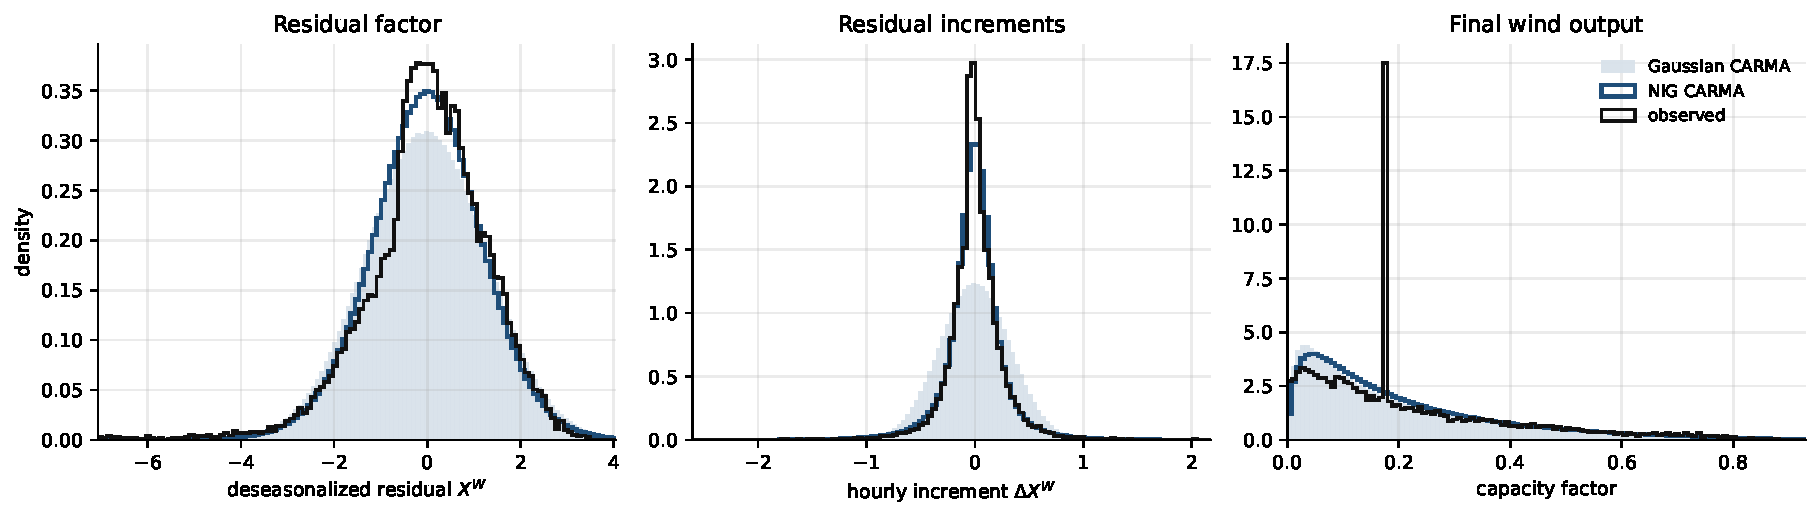
\includegraphics[width=0.97\textwidth]{calibration/wind_distribution_checks.pdf}
  \caption{Distribution checks for the German wind marginal model at the deseasonalized logit residual, hourly residual-increment, and physical capacity-factor levels.}
  \label{fig:app-wind-distribution-checks}
\end{figure}



\FloatBarrier


\clearpage
\section{Coupling Diagnostics}
\label{app:coupling-diagnostics}

The figures in this appendix compare the raw deseasonalized residual levels
with the projected state-space residuals used by the covariance estimator in
\cref{sec:coupling-calibration}. The raw plots describe visible marginal
co-movement, whereas the projected plots correspond to the CARMA state
residuals on which the coupling coefficient is estimated.

\begin{figure}[H]
  \centering
  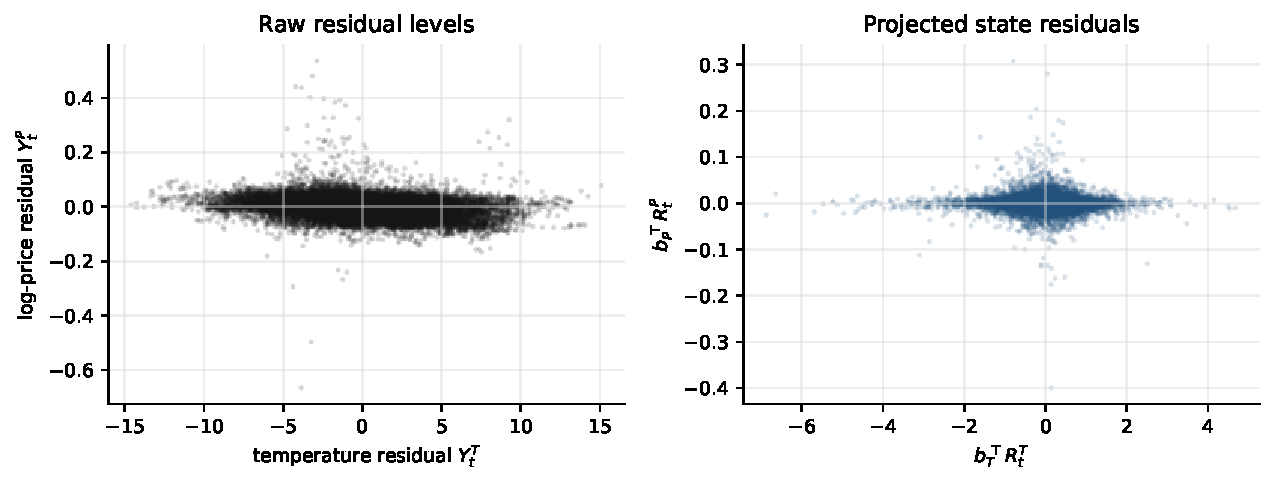
\includegraphics[width=0.97\textwidth]{appendix/coupling_temperature_scatter.pdf}
  \caption{Temperature--price residual scatter plots. The first panel uses raw
  deseasonalized residual levels. The second panel uses the projected
  state-space residuals entering the covariance-based coupling estimator.}
  \label{fig:app-temperature-coupling-scatter}
\end{figure}

\begin{figure}[H]
  \centering
  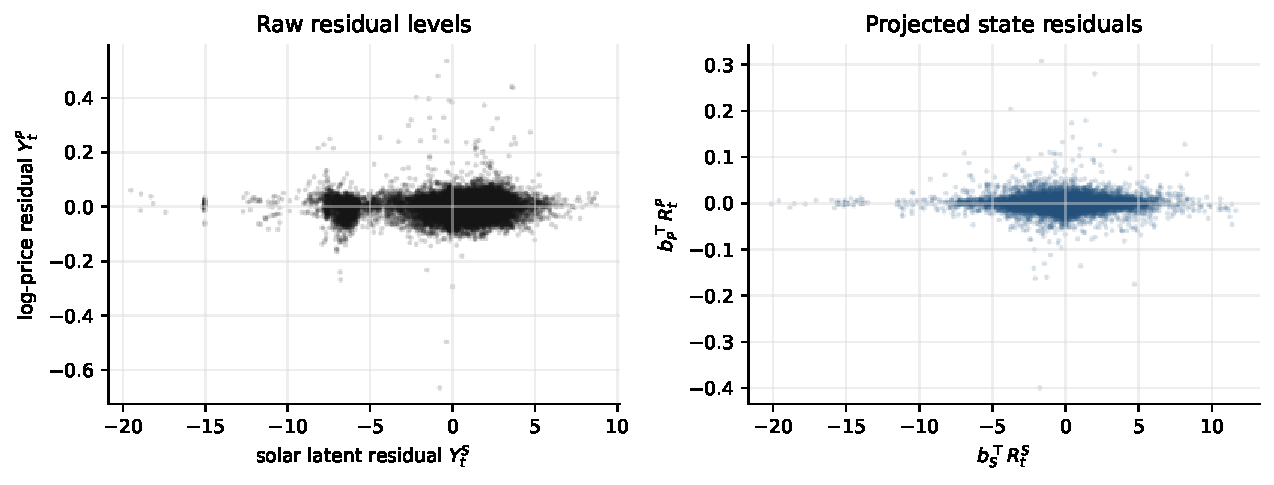
\includegraphics[width=0.97\textwidth]{appendix/coupling_solar_scatter.pdf}
  \caption{Solar--price residual scatter plots. The raw residual is the solar
  latent shortfall coordinate, while the projected residual is obtained from the
  calibrated CARMA state-space filter.}
  \label{fig:app-solar-coupling-scatter}
\end{figure}

\begin{figure}[H]
  \centering
  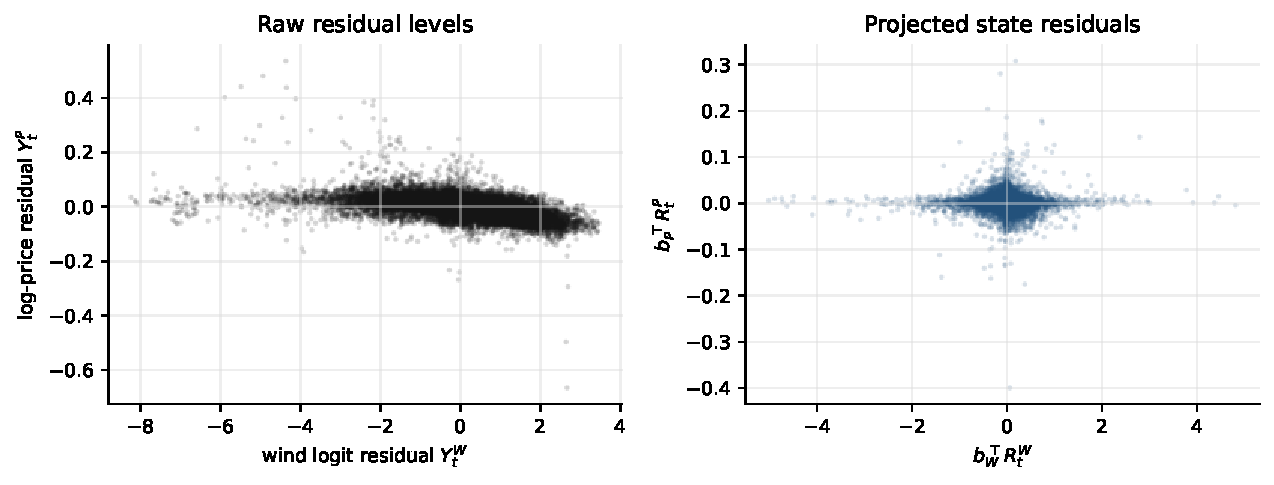
\includegraphics[width=0.97\textwidth]{appendix/coupling_wind_scatter.pdf}
  \caption{Wind--price residual scatter plots. The first panel uses wind logit
  residual levels and the second panel uses the corresponding projected CARMA
  state-space residuals.}
  \label{fig:app-wind-coupling-scatter}
\end{figure}

\FloatBarrier



\bibliographystyle{unsrtnat}
\bibliography{references}

\end{document}
